%% PREAMBLE %%%%%%%%%%%%%%%%%%%%%%%%%%%%%%%%%%%%%%%%%%%%%%%%%

\documentclass[11pt,a4paper,final,twoside]{memoir}

\newcommand{\thesisTitleMain}{Molecular signatures of survival in pancreatic ductal adenocarcinoma}
\newcommand{\thesisTitleSub}{why do some patients live longer than others, and how can we identify them?}
\newcommand{\thesisTitleSUB}{Why do some patients live longer than others, and how can we identify them?}
\newcommand{\thesisTitle}{\thesisTitleMain{}:~\\\thesisTitleSub{}}


% DRAFT STUFF -- TODO: REMOVE FOR FINAL
\overfullrule=2cm


% UNSW-mandated ugly
\settrimmedsize{297mm}{210mm}{*}
\settrims{0pt}{0pt}
\settypeblocksize{200mm}{115mm}{*}
\setbinding{10mm}
\setlrmargins{40mm}{*}{*}
\setulmargins{60mm}{*}{*}
\setheadfoot{2\onelineskip}{3\onelineskip}
\setheaderspaces{*}{2\onelineskip}{*}
\checkandfixthelayout

% CHOPPING N CUTTING
\usepackage{subfiles}

% VERSIONING
\usepackage{mVersion}

% FIXME
\usepackage[draft,footnote,nomargin]{fixme}   	% TODO TODO: Remove draft flag for final!
\FXRegisterAuthor{mp}{amp}{MP}
\FXRegisterAuthor{mjc}{amjc}{MJC}

\usepackage[table,xcdraw]{xcolor}

% ALGORITHMS
\usepackage{listings}
\usepackage{algorithm2e}

% MATHS
\usepackage{amsmath}
\let\equation\gather
\let\endequation\endgather
\usepackage{amssymb}
\usepackage{bm}

% TRADEMARK
\usepackage{textcomp}

% GRAPHICS
\usepackage{pdfpages}
\usepackage{graphicx}
\usepackage{tikz}
\usetikzlibrary{decorations.pathreplacing}

% CAPTIONS
\usepackage[singlelinecheck=off]{caption}		% To get left caption alignment on longtables

% CROSS-REFERENCING
\usepackage[colorlinks=true,hidelinks,plainpages=false,pdfpagelabels]{hyperref}

% GLOSSARY
\usepackage[toc,noredefwarn]{glossaries}
\let\originalgls\gls
\renewcommand{\gls}[1]{\ifglsentryexists{#1}{\originalgls{#1}}{\colorbox{red}{\underline{#1}}}}
\let\originalglspl\glspl
\renewcommand{\glspl}[1]{\ifglsentryexists{#1}{\originalglspl{#1}}{\colorbox{red}{\underline{#1}}}}
\let\originalGls\Gls
\renewcommand{\Gls}[1]{\ifglsentryexists{#1}{\originalGls{#1}}{\colorbox{red}{\underline{#1}}}}
\let\originalGlspl\Glspl
\renewcommand{\Glspl}[1]{\ifglsentryexists{#1}{\originalGlspl{#1}}{\colorbox{red}{\underline{#1}}}}

% SUBFIGURES
\newsubfloat{figure}		% AFTER hyperref!


\newcommand*{\approxdist}{\mathrel{\vcenter{\offinterlineskip
\vskip-.25ex\hbox{\hskip.55ex$\cdot$}\vskip-.25ex\hbox{$\sim$}
\vskip-.5ex\hbox{\hskip.55ex$\cdot$}}}}



\lstset{basicstyle=\footnotesize\ttfamily,breaklines=true}
\lstset{framextopmargin=50pt,frame=bottomline}
%\cleartoevenpage[\vspace*{\fill}This page intentionally left unblank\vspace*{\fill}]
%\cleartooddpage[\vspace*{\fill}This page intentionally left unblank\vspace*{\fill}]


\newacronym{HMM}{HMM}{hidden Markov model}
\newacronym{CNV}{CNV}{copy number variation}
\newacronym{LOH}{LOH}{loss of heterozygosity}
\newacronym{FDR}{FDR}{false-discovery rate}
\newacronym{BIC}{BIC}{Bayesian information criterion}
\newacronym{CPV}{CPV}{clinico-pathological variable}
\newacronym{SNV}{SNV}{single nucleotide variant}
\newacronym{LABQSR}{LA-BQSR}{local alignment and base quality score recalibration}
\newacronym{GATK}{GATK}{Genome analysis toolkit}
\newacronym{BAM}{BAM}{binary sequence alignment / map file}
\newacronym{indel}{indel}{insertion / deletion event}
\newacronym{BMC}{BMC}{Bayesian model comparison}
\newacronym{NGS}{NGS}{next-generation sequencing}
\newacronym{WGS}{WGS}{whole genome sequencing}
\newacronym{SNR}{SNR}{signal-to-noise ratio}
\newacronym{KDE}{KDE}{kernel density estimate}
\newacronym{MDS}{MDS}{multidimensional scaling}
\newacronym{IDAT}{IDAT}{Illumina data}
\newacronym{SIS}{SIS}{sure independence screening}
\newacronym{CPSS}{CPSS}{complementary pair subset selection}
\newacronym{FAST}{FAST}{feature aberration at survival times}
\newacronym{NMF}{NMF}{non-negative matrix factorization}
\newacronym{GEX}{GEX}{gene expression}
\newacronym{VST}{VST}{variance stabilizing transform}
\newacronym{GSVA}{GSVA}{gene set variation analysis}
\newacronym{SNMFL}{SNMF/L}{sparse non-negative matrix factorization, long variant}
\newacronym{MSigDB}{MSigDB}{molecular signatures database}
\newacronym{LASSO}{LASSO}{least absolute shrinkage and selection operator}
\newacronym{EMT}{EMT}{epithelial to mesenchymal transition}
\newacronym{NNLS}{NNLS}{non-negative least squares}
\newacronym{APGI}{APGI}{Australian Pancreatic Cancer Genome Initiative}
\newacronym{PDAC}{PDAC}{pancreatic ductal adenocarcinoma}
\newacronym{NCBI}{NCBI}{National Center for Biotechnology Information}
\newacronym{GEO}{GEO}{Gene Expression Omnibus}
\newacronym{BH}{BH}{Benjamini-Hochberg}

\makeglossaries

\begin{document}
\pagestyle{empty}
\hypersetup{pageanchor=false}	% Disable page number anchors in hyperref for early
								% pages, to prevent duplicate page warnings.
\raggedbottom

%\listoffixmes

\begin{tikzpicture}[remember picture,overlay,shift={(current page.center)}]
    \node at (0.8cm,0) (OffsetNode) {};
\end{tikzpicture}
\begin{tikzpicture}[remember picture,overlay,shift={(OffsetNode.center)}]
    \node at (0,0) {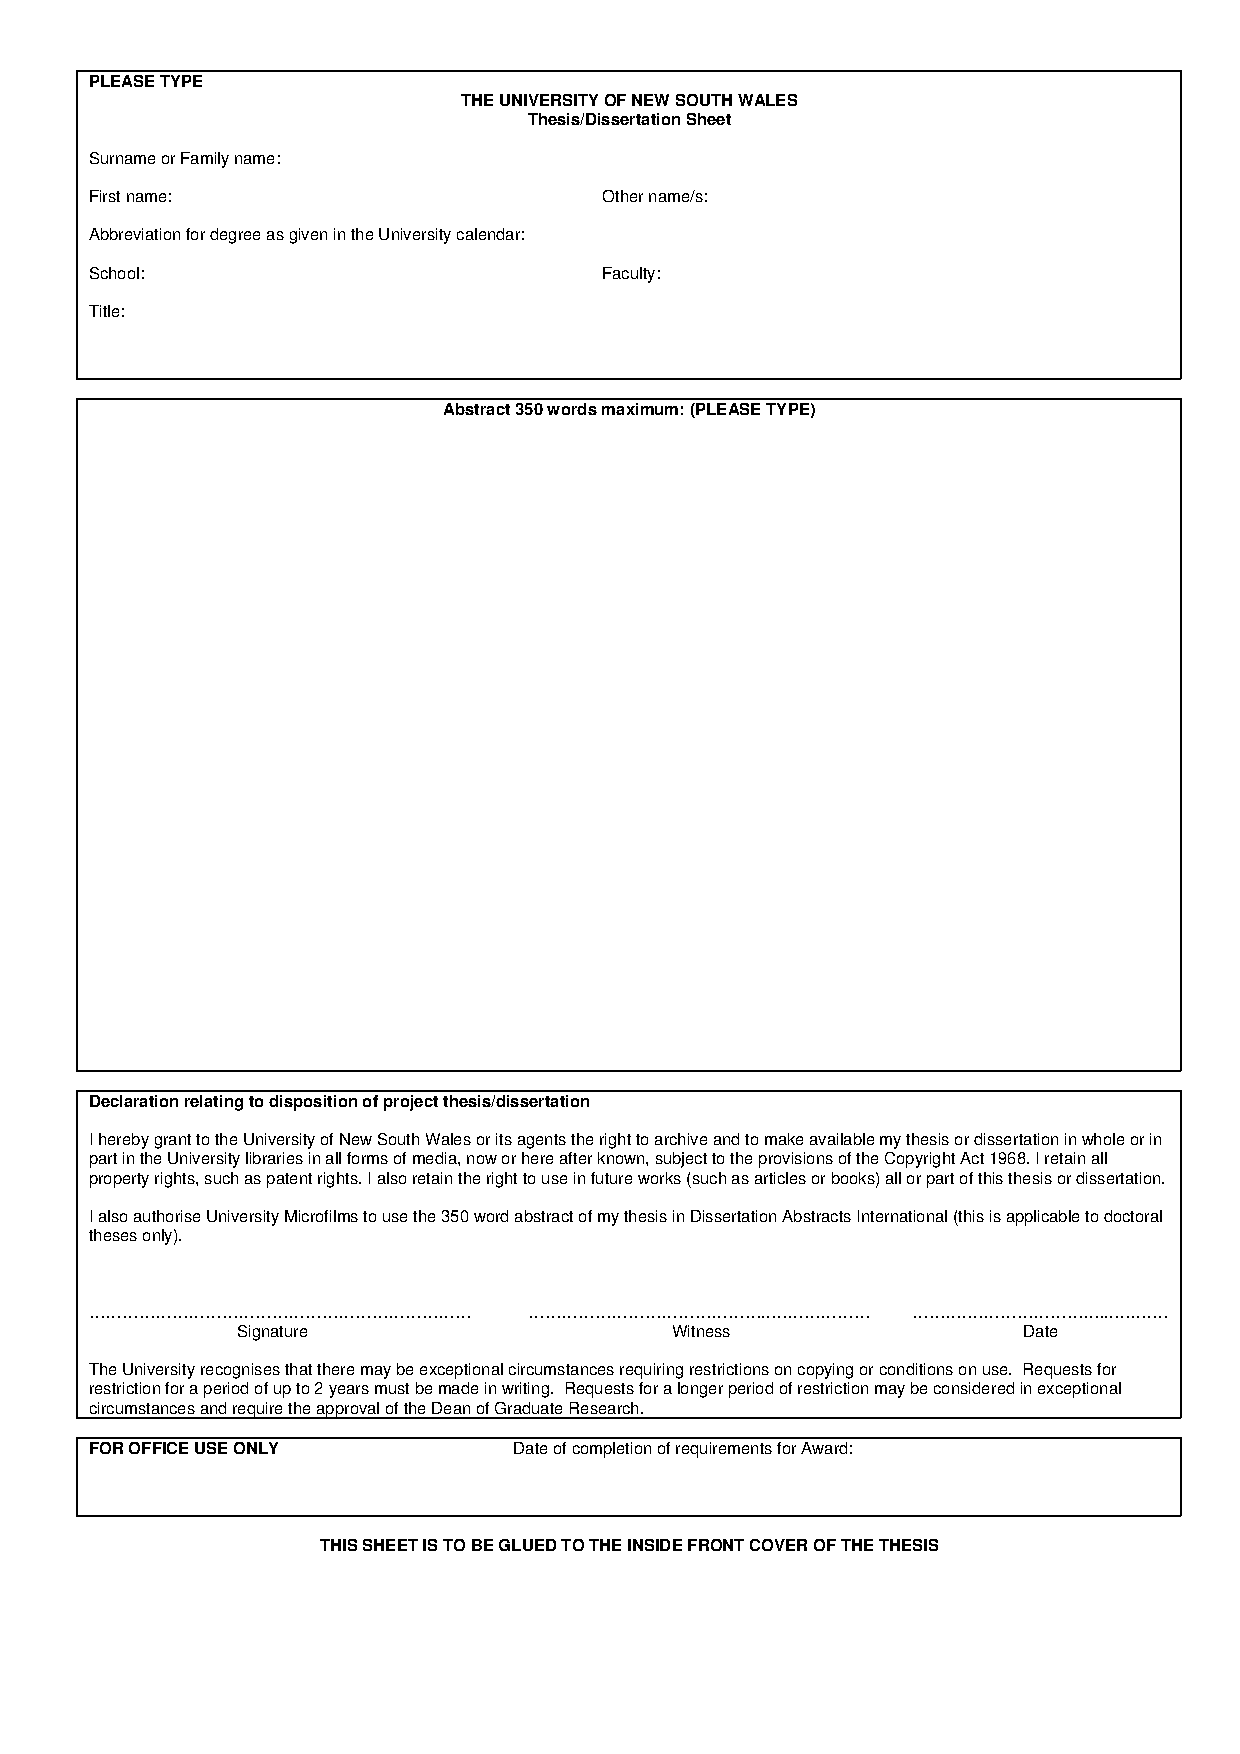
\includegraphics[page=1,scale=0.8]{resources/thesisdissertation}};
    \begin{scope}[shift={(current page.south west)},every node/.style={anchor=base west}]
%        \draw [help lines] (0,0) grid (current page.north east);
%        \draw [help lines,thick] (0,0) grid [step=5cm] (current page.north east);
        \node[font=\scriptsize] at (7cm,24.5cm)	{Pinese};
        \node[font=\scriptsize] at (7cm,24cm) 	{Mark};
        \node[font=\scriptsize] at (11cm,23.48cm) {PhD};
        \node[font=\scriptsize] at (7cm,22.95cm) 	{St. Vincent's Clinical School};
        \node[text width=13cm,align=left,text ragged,font=\scriptsize] at (5cm,22.4cm) 	{\thesisTitle{}};
        \node[font=\scriptsize] at (13cm,22.95cm)	{Medicine};
        \node[text width=13.5cm,align=left,font=\tiny] at (4.5cm,20.5cm)	{\setlength{\parskip}{2.5mm} \noindent \noindent Pancreatic ductal adenocarcinoma (PDAC) is the most deadly common cancer, with fewer than ten percent of patients surviving five years from diagnosis.  In contrast to many other cancers, the grim prognosis of PDAC has remained largely the same over the past thirty years, reflecting our relatively poor understanding of the disease.  This situation may soon change: recent large-scale efforts have produced detailed molecular and clinical data for almost a thousand cases of PDAC, finally enabling detailed dissection of the cancer's molecular basis.  This work used these new data to directly address two questions linked to PDAC's exceptionally poor prognosis: what are the biological processes that drive poor prognosis in PDAC? and can we develop a practical and effective prognostic staging system to better guide PDAC treatment?
\par
\Cref{chap:signatures} considered the first question, using a gene expression factorization approach to identify two metagenes that determine survival in PDAC.  These metagenes were linked to the biological processes of proliferation, and the EMT, and were also prognostic in a number of other solid tumours, revealing these processes as generally important to cancer patient survival.  
\par
\Cref{chap:nomogram} addressed the second question, developing a pilot tool to estimate the prognosis of a PDAC patient, and guide the decision of whether to resect that patient's tumour.  The tool is unique in that it can be applied prior to resection, and its validation performance was competitive with gold standard post-resection methods.  This performance might be improved through better selection of prognostic biomarkers; this is the subject of \Cref{chap:messina}, which describes a method for the identification of biomarkers that are well-suited for development into clinical tests.
\par
PDAC has an exceptionally poor prognosis, but better understanding of the disease, and improvements in its management, can yield incrementally better outcomes.  The work presented here focussed on understanding and predicting prognosis in PDAC.  It identified two metagenes that were strongly linked to outcome, indicating valuable therapeutic directions to improve the survival of patients with particularly aggressive tumours; and it provided a proof-of-concept, and a method for development, of a biomarker-based preoperative prognostic tool for the improved management of PDAC.
};
    \end{scope}
\end{tikzpicture}

\increaseBuild
\cleardoublepage

\begin{titlingpage}
    \begin{center}
        \vspace*{1cm}
        
        \Large
        \textbf{\thesisTitleMain{}}
        
        \vspace{1cm}
        \normalsize
        \textbf{\thesisTitleSUB{}}
        
        \vspace{2.25cm}
        
        \normalsize
        \textbf{Mark Pinese}
        
        \vfill
        
        A thesis in fulfilment of the requirements for the degree of\\
        Doctor of Philosophy
        
        \vspace{3cm}
        
        
\includegraphics[width=0.25\textwidth]{resources/PortraitColourPos}

        \vspace{1.5cm}

        St. Vincent's Clinical School\\
        Faculty of Medicine\\

		\vspace{1.2cm}
        March 2015
    \end{center}
\end{titlingpage}


\cleardoublepage
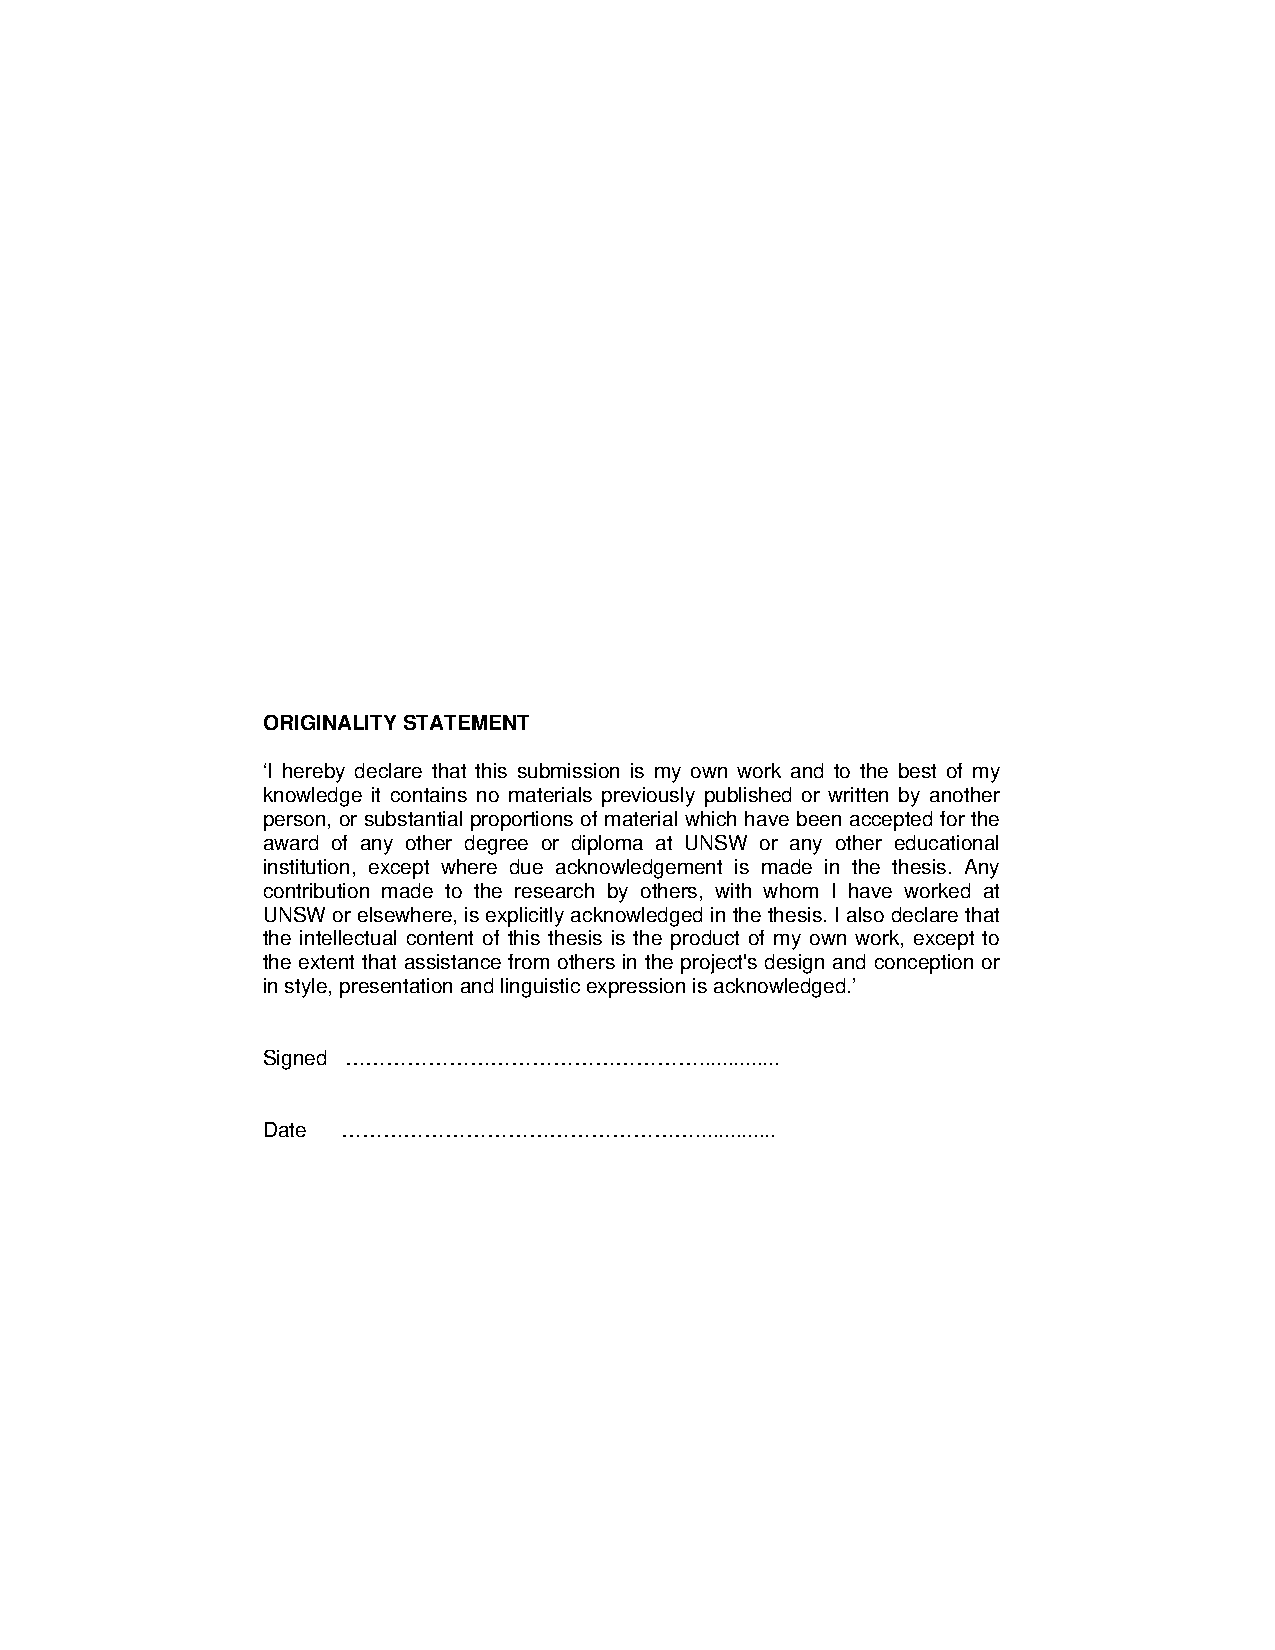
\includepdf[pages={1},lastpage=1]{resources/originalitystatement_1.pdf}

\frontmatter

\cleardoublepage
\vspace*{\stretch{3}}
\begin{adjustwidth}{2em}{2em}
%\centering
\noindent
To Emma and Eva -- ~\\
\hspace{1cm}it's done now!
\end{adjustwidth}
\vspace*{\stretch{11}}

\chapter*{Acknowledgements}
As tempted as I was at times to follow the path of Shivers' outstanding non-acknowledgement \cite{Shivers1994}, in truth this work would simply not be without the myriad contributions of friends, family, and colleagues.

I am indebted to Prof. Andrew Biankin, for teaching me some of the rules of professional science, and for his great accomplishment in piloting the \acrshort{APGI} to success; without the data generated by that project, this dissertation would not have been possible.  Likewise, Prof. Sean Grimmond and his group at the Institute of Molecular Bioscience were instrumental in generating the lion's share of the expression data upon which I worked.

Survival analysis requires exacting interpretation, coding, and follow-up of clinical records; laborious and difficult work that is too often left unacknowledged.  I am very grateful to the entire clinical data team of the \acrshort{APGI}/\acrshort{NSWPCN}, for thanklessly collating the high-quality data which I required, and for humouring my continual requests for data.  In particular, this work would be far weaker without the substantial contributions of Clare Watson, Skye Simpson, Mary-Anne Brancato, and Amber Johns.

Dr. David Chang taught me so much about true translational research; his work and guidance continues to transform the predictor of Chapter 3 from an academic exercise, into something that could truly make a positive difference for patients.  His contributions to the greater prognostic predictor project far outweigh mine, and his long efforts on molecular prognostics in pancreas cancer enabled the small work I describe here.

Dr. Mark Cowley, I suspect, was not quite aware of the task ahead when he kindly agreed to supervise me following Prof. Biankin's departure.  This dissertation is stronger for his critical input, and his patient help and encouragement at all times was far better than I think I deserved.

Friends and family have given support, both overt and covert, freely through the last four years.  In particular, Aaron Statham, Alison Ferguson, and Drs. Hugh French and Brian Gloss, have made contributions to my mental health -- usually administered at Darlo Bar -- that go beyond the call of duty.  I have also been very fortunate to have had the unquestioning support of the Pinese and Scott families.

Scholarships from the Australian government, UNSW Australia, and the Garvan Institute meant that I did not need to cut back on my food habit in order to meet my basic coffee needs.

Too many people have assisted this work, directly or indirectly, for me to list them all here.  To all of these, I apologise if I have omitted you -- remind me sometime, and I promise you a drink of your choice.  Some I suspect have been assisting in secret.  To those, you really should have seen this omission coming, but thanks all the same.

It's traditional to save the best to last; in this case it's also amusing.  To my truly amazing wife Emma: thank you.  Though you didn't write a word, I see this dissertation as much your work as mine.  Throughout this PhD, you have shown fortitude and compassion that is inspirational.  I probably will never know all the secret machinations that you undertook to make this dissertation happen -- at least not until I receive an itemized bill -- but I want you to know that they worked, and that this simply wouldn't have come together without you.  And to little Eva: you just might read this some day, so you may as well know that you were a very early overachiever -- you gave Dad a great big kick up the arse, even when you were less than two feet tall!

\vspace{15mm}

\hspace{70mm}Sydney

\hspace{70mm}23 March 2015


\thispagestyle{empty}
\clearpage

\begin{abstract}
\noindent Pancreatic ductal adenocarcinoma (PDAC) is the most deadly common cancer, with fewer than ten percent of patients surviving five years from diagnosis.  In contrast to many other cancers, the grim prognosis of PDAC has remained largely the same over the past thirty years, reflecting our relatively poor understanding of the disease.  This situation may soon change: recent large-scale efforts have produced detailed molecular and clinical data for almost a thousand cases of PDAC, finally enabling detailed dissection of the cancer's molecular basis.  This work used these new data to directly address two questions linked to PDAC's exceptionally poor prognosis: what are the biological processes that drive poor prognosis in PDAC? and can we develop a practical and effective prognostic staging system to better guide PDAC treatment?
\par
\Cref{chap:signatures} considered the first question, using a gene expression factorization approach to identify two metagenes that determine survival in PDAC.  These metagenes were linked to the biological processes of proliferation, and the EMT, and were also prognostic in a number of other solid tumours, revealing these processes as generally important to cancer patient survival.  
\par
\Cref{chap:nomogram} addressed the second question, developing a pilot tool to estimate the prognosis of a PDAC patient, and guide the decision of whether to resect that patient's tumour.  The tool is unique in that it can be applied prior to resection, and its validation performance was competitive with gold standard post-resection methods.  This performance might be improved through better selection of prognostic biomarkers; this is the subject of \Cref{chap:messina}, which describes a method for the identification of biomarkers that are well-suited for development into clinical tests.
\par
PDAC has an exceptionally poor prognosis, but better understanding of the disease, and improvements in its management, can yield incrementally better outcomes.  The work presented here focussed on understanding and predicting prognosis in PDAC.  It identified two metagenes that were strongly linked to outcome, indicating valuable therapeutic directions to improve the survival of patients with particularly aggressive tumours; and it provided a proof-of-concept, and a method for development, of a biomarker-based preoperative prognostic tool for the improved management of PDAC.

\end{abstract}
\thispagestyle{empty}
\pagenumbering{gobble}
\clearpage

\OnehalfSpacing
%\DoubleSpacing

\hypersetup{pageanchor=true}		% Re-enable page numbering
\pagenumbering{roman}
\chapterstyle{brotherton}

\setcounter{tocdepth}{2}
\tableofcontents
\clearpage

\openany
\listoffigures
\clearpage

\listoftables
\clearpage

\addcontentsline{toc}{chapter}{List of Algorithms}
\listofalgorithms

\chapter*{Software Versions}
\addcontentsline{toc}{chapter}{Software Versions}
The following versions of software were used in all work.

\begin{ctabular}{ll}
\toprule
  MSigDB                      & 4.0 \\
%  Python                      & 2.7.8 / 3.4.1 \\
  R                           & 3.1.1 \\
  \quad ahaz                  & 1.14 \\
  \quad doMC                  & 1.3.3 \\
  \quad energy                & 1.6.2 \\
  \quad Exact                 & 1.4 \\
  \quad flexsurv              & 0.5 \\
  \quad GSVA                  & 1.14.1 \\
  \quad illuminaHumanv4.db    & 1.24.0 \\
  \quad lumi                  & 2.18.0 \\
  \quad lumidat               & 1.2.3 \\
  \quad MASS                  & 7.3-35 \\
  \quad maxstat               & 0.7-22 \\
%  \quad muhaz                 & 1.2.6 \\
  \quad NMF                   & 0.20.5 \\
  \quad nnls                  & 1.4 \\
  \quad randomForestSRC       & 1.5.5 \\
  \quad risksetROC            & 1.0.4 \\
  \quad robustbase            & 0.92-3 \\
%  \quad survcomp              & 1.16.0 \\
  \quad survival              & 2.37-7 \\
  \quad shiny                 & 0.10.2.2 \\
\bottomrule
\end{ctabular}


\chapter*{Conventions}
Unless otherwise specified, the following conventions are used throughout this dissertation.

\begin{itemize}
  \item Indices in algorithm pseudocode are 1-based.
  \item Logarithms ($\log$) and exponentiations ($\exp$) are to base $e$.
  \item Square brackets around a predicate $P$ denote the Iverson bracket: $\left[P\right] \Leftrightarrow 1\ \mathrm{if}\ P \mathrm{~is~true,~else}\ 0$.
  \item Square brackets around a function-predicate pair $f(i)~|~P(i)$, indicate tuple builder notation: $\left[f(i)~|~P(i)\right]_{i=a}^b \Leftrightarrow \left[ f(a), f(a+1), \dots, f(b) \right]$, where an element $f(i)$ is only included in the tuple if $P(i)$ is true.
  \item $x_+$ indicates the value of the ramp function at real $x$, $x_+ := \max(0, x)$.
  \item $\mathbf{0}^n$ denotes the vector in $\mathbf{R}^n$ with all entries equal to zero.
  \item $\mathbb{B}$ denotes the Boolean set $\{true, false\}$.
\end{itemize}


\mainmatter
\openright
\pagestyle{headings}

\subfile{introduction}
\subfile{signatures}
\subfile{nomogram}
\subfile{messina}
\subfile{conclusion}

\appendix
\appendixpage*
\addappheadtotoc

\chapter{Basis matrix \texorpdfstring{$W$}{W} for the six survival-associated metagenes}
\label{app:sigs-w-matrix}
% latex table generated in R 3.1.1 by xtable 1.7-4 package
% Fri Dec  5 15:39:01 2014
\begin{longtable}{rrrrrrr}
  \hline
 & 1 & 2 & 3 & 4 & 5 & 6 \\ 
  \hline
PPY & 0.00 & 0.50 & 0.00 & 0.08 & 1.08 & 0.00 \\ 
  KRT6A & 0.14 & 0.00 & 0.12 & 0.00 & 0.00 & 0.47 \\ 
  KRT17 & 0.29 & 0.00 & 0.39 & 0.16 & 0.12 & 0.51 \\ 
  DHRS9 & 0.00 & 0.00 & 1.00 & 0.34 & 0.00 & 0.17 \\ 
  SPP1 & 0.03 & 0.08 & 0.00 & 1.04 & 0.31 & 0.74 \\ 
  ADH1A & 0.07 & 0.44 & 0.01 & 0.10 & 0.66 & 0.00 \\ 
  IGLL3P & 0.17 & 0.15 & 0.00 & 0.00 & 0.76 & 0.00 \\ 
  DKK1 & 0.48 & 0.00 & 0.30 & 0.18 & 0.00 & 0.02 \\ 
  APCS & 0.00 & 0.03 & 0.16 & 0.10 & 0.16 & 0.35 \\ 
  CST6 & 0.07 & 0.00 & 0.20 & 0.00 & 0.07 & 0.63 \\ 
  ANGPTL4 & 0.18 & 0.00 & 0.42 & 0.05 & 0.03 & 0.39 \\ 
  KRT7 & 0.46 & 0.00 & 0.56 & 0.00 & 0.14 & 0.44 \\ 
  PLAU & 0.21 & 0.00 & 0.28 & 0.00 & 0.02 & 0.88 \\ 
  SCGB2A1 & 0.00 & 0.83 & 0.00 & 0.18 & 0.15 & 0.00 \\ 
  CCL19 & 0.00 & 0.00 & 0.00 & 0.00 & 0.95 & 0.00 \\ 
  CYP2S1 & 0.32 & 1.02 & 0.15 & 0.00 & 0.09 & 0.00 \\ 
  SLC2A1 & 0.18 & 0.12 & 1.00 & 0.41 & 0.00 & 0.70 \\ 
  ADM & 0.00 & 0.00 & 0.52 & 0.51 & 0.00 & 0.36 \\ 
  FAM83A & 0.25 & 0.00 & 0.12 & 0.00 & 0.00 & 0.22 \\ 
  FGG & 0.05 & 0.04 & 0.00 & 0.14 & 0.01 & 0.22 \\ 
  KRT6C & 0.12 & 0.00 & 0.00 & 0.00 & 0.00 & 0.16 \\ 
  PHACTR3 & 0.15 & 0.00 & 0.32 & 0.14 & 0.00 & 0.07 \\ 
  C9orf152 & 0.21 & 1.37 & 0.00 & 0.35 & 0.02 & 0.00 \\ 
  ALOX5AP & 0.05 & 0.01 & 0.01 & 1.27 & 0.34 & 0.71 \\ 
  DCBLD2 & 0.40 & 0.00 & 0.12 & 0.00 & 0.14 & 0.84 \\ 
  CIDEC & 0.03 & 0.00 & 0.43 & 0.28 & 0.00 & 0.00 \\ 
  FGB & 0.00 & 0.00 & 0.02 & 0.32 & 0.00 & 0.08 \\ 
  SERPINB3 & 0.00 & 0.00 & 0.18 & 0.18 & 0.00 & 0.05 \\ 
  SLC16A3 & 0.13 & 0.38 & 1.10 & 0.42 & 0.00 & 1.00 \\ 
  FST & 0.00 & 0.00 & 0.16 & 0.00 & 0.04 & 0.49 \\ 
  CAV1 & 0.42 & 0.00 & 0.19 & 0.08 & 0.27 & 0.84 \\ 
  TGFBI & 0.19 & 0.00 & 0.15 & 0.19 & 0.05 & 1.00 \\ 
  COL12A1 & 0.00 & 0.13 & 0.03 & 0.53 & 0.19 & 1.65 \\ 
  SLC2A3 & 0.00 & 0.00 & 0.34 & 0.76 & 0.33 & 0.72 \\ 
  SUGCT & 0.00 & 0.03 & 0.00 & 0.63 & 0.13 & 0.93 \\ 
  IL1R2 & 0.04 & 0.25 & 0.43 & 0.23 & 0.00 & 0.06 \\ 
  TCEA3 & 0.00 & 0.89 & 0.26 & 0.09 & 0.62 & 0.00 \\ 
  RAP1GAP & 0.00 & 1.01 & 0.47 & 0.28 & 0.75 & 0.00 \\ 
  PXDN & 0.00 & 0.00 & 0.38 & 0.59 & 0.31 & 1.19 \\ 
  FRZB & 0.09 & 0.24 & 0.00 & 0.54 & 1.50 & 0.00 \\ 
  IL20RB & 0.26 & 0.00 & 0.31 & 0.00 & 0.00 & 0.68 \\ 
  PLEKHS1 & 0.00 & 0.64 & 0.34 & 0.09 & 0.28 & 0.02 \\ 
  HSPB6 & 0.00 & 0.15 & 0.13 & 0.00 & 1.31 & 0.31 \\ 
  KANK4 & 0.00 & 0.00 & 0.20 & 0.47 & 0.00 & 1.23 \\ 
  COL7A1 & 0.00 & 0.00 & 0.59 & 0.00 & 0.00 & 0.59 \\ 
  C5orf46 & 0.00 & 0.00 & 0.00 & 1.06 & 0.13 & 1.04 \\ 
  VSTM2L & 0.32 & 0.00 & 0.94 & 0.00 & 0.05 & 0.07 \\ 
  PTGES & 0.57 & 0.02 & 0.57 & 0.07 & 0.00 & 0.56 \\ 
  FSCN1 & 0.37 & 0.07 & 1.06 & 0.13 & 0.14 & 0.74 \\ 
  CTSV & 0.30 & 0.04 & 0.26 & 0.02 & 0.02 & 0.18 \\ 
  SPOCK1 & 0.12 & 0.00 & 0.03 & 0.52 & 0.34 & 1.27 \\ 
  RGS5 & 0.00 & 0.43 & 0.05 & 0.08 & 0.58 & 0.09 \\ 
  PHLDA1 & 0.08 & 0.14 & 0.72 & 0.13 & 0.62 & 1.50 \\ 
  IGFBP1 & 0.27 & 0.00 & 0.23 & 0.03 & 0.00 & 0.01 \\ 
  BAMBI & 0.11 & 0.00 & 0.84 & 0.39 & 0.24 & 0.17 \\ 
  FLRT3 & 0.79 & 0.13 & 0.51 & 0.28 & 0.22 & 0.31 \\ 
  DSG3 & 0.18 & 0.00 & 0.21 & 0.00 & 0.00 & 0.54 \\ 
  ANGPTL2 & 0.00 & 0.00 & 0.37 & 0.87 & 0.18 & 0.92 \\ 
  ST6GAL1 & 0.17 & 0.84 & 0.00 & 0.23 & 0.67 & 0.09 \\ 
  SLC40A1 & 0.00 & 0.89 & 0.00 & 0.58 & 0.24 & 0.16 \\ 
  EMP3 & 0.25 & 0.00 & 0.46 & 0.16 & 0.22 & 0.56 \\ 
  RAB31 & 0.11 & 0.00 & 0.26 & 0.87 & 0.76 & 1.19 \\ 
  ST6GALNAC1 & 0.04 & 1.00 & 0.08 & 0.12 & 0.00 & 0.10 \\ 
  ACKR3 & 0.00 & 0.00 & 0.38 & 0.36 & 0.21 & 0.58 \\ 
  SLC12A2 & 0.04 & 0.91 & 0.34 & 0.10 & 0.49 & 0.18 \\ 
  ANKRD22 & 0.41 & 1.35 & 0.17 & 0.27 & 0.04 & 0.22 \\ 
  ENO2 & 0.36 & 0.34 & 0.79 & 0.03 & 0.00 & 0.94 \\ 
  EPHX2 & 0.00 & 0.59 & 0.11 & 0.17 & 0.68 & 0.00 \\ 
  MCEMP1 & 0.00 & 0.00 & 0.00 & 0.61 & 0.00 & 0.30 \\ 
  CDA & 0.29 & 0.00 & 0.34 & 0.00 & 0.00 & 0.70 \\ 
  PLIN2 & 0.31 & 0.00 & 0.08 & 1.02 & 0.47 & 0.21 \\ 
  SERPINH1 & 0.00 & 0.01 & 0.39 & 0.22 & 0.43 & 1.02 \\ 
  FAM134B & 0.00 & 0.82 & 0.00 & 0.23 & 0.21 & 0.00 \\ 
  NFIX & 0.00 & 0.88 & 0.14 & 0.00 & 1.39 & 0.80 \\ 
  LYNX1 & 0.03 & 0.00 & 0.26 & 0.17 & 0.00 & 0.10 \\ 
  LDHA & 0.65 & 0.47 & 0.00 & 0.32 & 0.05 & 1.17 \\ 
  SOD2 & 0.58 & 0.12 & 0.00 & 0.47 & 0.40 & 0.17 \\ 
  PCDH20 & 0.00 & 0.43 & 0.00 & 0.15 & 0.00 & 0.00 \\ 
  ITGA5 & 0.00 & 0.00 & 0.48 & 0.27 & 0.12 & 0.68 \\ 
  ZNF185 & 0.25 & 0.17 & 1.02 & 0.48 & 0.00 & 0.72 \\ 
  PLOD2 & 0.15 & 0.09 & 0.24 & 0.29 & 0.17 & 0.89 \\ 
  TNFRSF6B & 0.63 & 0.00 & 0.07 & 0.18 & 0.00 & 0.39 \\ 
  MME & 0.00 & 0.00 & 0.06 & 0.45 & 0.04 & 0.58 \\ 
  MRAP2 & 0.04 & 0.78 & 0.00 & 0.22 & 0.23 & 0.00 \\ 
  PLAC9 & 0.07 & 0.00 & 0.00 & 0.11 & 1.29 & 0.08 \\ 
  ERRFI1 & 0.16 & 0.03 & 0.55 & 0.35 & 0.29 & 0.79 \\ 
  PP7080 & 0.10 & 0.97 & 0.00 & 0.04 & 0.00 & 0.00 \\ 
  DSG2 & 0.43 & 0.57 & 0.18 & 0.51 & 0.04 & 0.71 \\ 
  APCDD1 & 0.00 & 0.14 & 0.15 & 0.13 & 0.60 & 0.84 \\ 
  PRKCDBP & 0.26 & 0.00 & 1.02 & 0.51 & 0.26 & 0.59 \\ 
  SULF2 & 0.17 & 0.15 & 0.46 & 0.19 & 0.39 & 0.77 \\ 
  TUBA1C & 1.31 & 0.55 & 0.54 & 0.53 & 0.27 & 0.50 \\ 
  PCOLCE2 & 0.00 & 0.01 & 0.12 & 0.54 & 0.00 & 0.05 \\ 
  LAMA5 & 0.37 & 0.08 & 1.02 & 0.00 & 0.34 & 0.18 \\ 
  P4HA1 & 0.04 & 0.10 & 0.41 & 0.84 & 0.00 & 0.55 \\ 
  RASL11B & 0.00 & 0.19 & 0.07 & 0.22 & 1.21 & 0.31 \\ 
  KYNU & 0.61 & 0.09 & 0.07 & 0.54 & 0.00 & 0.28 \\ 
  CTSL & 0.39 & 0.00 & 0.20 & 1.18 & 0.47 & 0.22 \\ 
  MARCKSL1 & 0.15 & 1.34 & 0.30 & 0.00 & 0.00 & 0.26 \\ 
  PRC1 & 0.96 & 0.35 & 0.04 & 0.04 & 0.00 & 0.32 \\ 
  C1QTNF6 & 0.00 & 0.00 & 0.59 & 0.62 & 0.22 & 0.97 \\ 
  CCR7 & 0.06 & 0.00 & 0.00 & 0.00 & 1.05 & 0.00 \\ 
  HRASLS2 & 0.33 & 0.00 & 0.30 & 0.22 & 0.00 & 0.00 \\ 
  CHN2 & 0.00 & 0.50 & 0.00 & 0.34 & 0.44 & 0.00 \\ 
  PYGL & 0.08 & 0.00 & 0.31 & 0.34 & 0.14 & 0.74 \\ 
  MELK & 1.02 & 0.29 & 0.00 & 0.23 & 0.01 & 0.22 \\ 
  LOX & 0.21 & 0.00 & 0.08 & 0.39 & 0.09 & 0.92 \\ 
  CDC45 & 0.96 & 0.08 & 0.11 & 0.34 & 0.03 & 0.00 \\ 
  AXIN2 & 0.00 & 0.52 & 0.44 & 0.13 & 0.81 & 0.29 \\ 
  ATL3 & 0.64 & 0.03 & 0.16 & 0.49 & 0.25 & 0.29 \\ 
  CAMK1G & 0.09 & 0.24 & 0.00 & 0.03 & 0.88 & 0.00 \\ 
  ABLIM1 & 0.01 & 0.91 & 0.32 & 0.00 & 0.61 & 0.34 \\ 
  TRIM2 & 0.13 & 1.15 & 0.31 & 0.31 & 0.36 & 0.00 \\ 
  TWIST1 & 0.00 & 0.00 & 0.20 & 0.91 & 0.12 & 1.20 \\ 
  ARSD & 0.15 & 1.24 & 0.19 & 0.00 & 0.22 & 0.14 \\ 
  CEBPB & 0.07 & 0.07 & 1.29 & 0.53 & 0.51 & 0.81 \\ 
  CEP55 & 1.42 & 0.33 & 0.00 & 0.17 & 0.00 & 0.46 \\ 
  GINS2 & 1.08 & 0.18 & 0.39 & 0.07 & 0.00 & 0.00 \\ 
  MCM4 & 1.28 & 0.14 & 0.31 & 0.03 & 0.01 & 0.13 \\ 
  PPP1R3C & 0.00 & 0.02 & 0.13 & 0.37 & 0.03 & 0.26 \\ 
  MTRNR2L1 & 0.28 & 0.56 & 0.49 & 0.07 & 0.55 & 0.00 \\ 
  CDK12 & 0.19 & 0.28 & 0.00 & 0.08 & 0.83 & 0.00 \\ 
  BIRC5 & 1.38 & 0.17 & 0.37 & 0.55 & 0.00 & 0.24 \\ 
  SPHK1 & 0.26 & 0.00 & 0.27 & 0.09 & 0.62 & 1.41 \\ 
  A4GALT & 0.03 & 0.00 & 1.30 & 0.08 & 0.36 & 0.52 \\ 
  ICAM2 & 0.50 & 0.20 & 0.48 & 0.31 & 0.40 & 0.13 \\ 
  ANKRD37 & 0.06 & 0.18 & 0.22 & 0.72 & 0.01 & 0.57 \\ 
  STK39 & 0.15 & 1.00 & 0.24 & 0.14 & 0.08 & 0.12 \\ 
  ASPM & 1.17 & 0.39 & 0.20 & 0.17 & 0.04 & 0.04 \\ 
  PFKFB4 & 0.55 & 0.22 & 0.68 & 0.43 & 0.14 & 0.29 \\ 
  IDH2 & 0.71 & 0.43 & 0.40 & 0.21 & 0.33 & 0.23 \\ 
  SGSM1 & 0.00 & 0.93 & 0.08 & 0.02 & 0.84 & 0.00 \\ 
  SELENBP1 & 0.00 & 1.20 & 0.36 & 0.20 & 0.26 & 0.00 \\ 
  P4HA2 & 0.32 & 0.17 & 0.12 & 0.54 & 0.11 & 0.74 \\ 
  LMO3 & 0.00 & 0.11 & 0.00 & 0.01 & 1.18 & 0.01 \\ 
  KLHL5 & 0.42 & 0.16 & 0.00 & 0.35 & 0.70 & 1.14 \\ 
  HIPK2 & 0.26 & 1.25 & 0.07 & 0.24 & 0.52 & 0.00 \\ 
  NAMPT & 0.34 & 0.00 & 0.05 & 0.75 & 0.32 & 0.35 \\ 
  NCAPG & 1.61 & 0.44 & 0.00 & 0.00 & 0.00 & 0.52 \\ 
  PLOD1 & 0.06 & 0.00 & 1.21 & 0.75 & 0.37 & 0.80 \\ 
  C2orf70 & 0.11 & 1.09 & 0.02 & 0.00 & 0.00 & 0.00 \\ 
  RERGL & 0.24 & 0.00 & 0.00 & 0.11 & 1.18 & 0.00 \\ 
  CFDP1 & 0.35 & 0.55 & 0.74 & 0.67 & 0.00 & 0.26 \\ 
  RACGAP1 & 1.37 & 0.37 & 0.14 & 0.19 & 0.07 & 0.33 \\ 
  SNRPB & 0.99 & 0.08 & 0.41 & 0.90 & 0.02 & 0.00 \\ 
  CLEC3B & 0.06 & 0.07 & 0.12 & 0.01 & 0.81 & 0.00 \\ 
  ANLN & 1.17 & 0.24 & 0.08 & 0.08 & 0.00 & 0.72 \\ 
  ZFPM1 & 0.00 & 1.22 & 0.29 & 0.00 & 0.43 & 0.15 \\ 
  UPP1 & 0.55 & 0.00 & 0.79 & 0.43 & 0.16 & 0.11 \\ 
  AURKB & 1.00 & 0.11 & 0.14 & 0.00 & 0.01 & 0.00 \\ 
  SYNE2 & 0.00 & 0.88 & 0.24 & 0.00 & 0.28 & 0.28 \\ 
  SOBP & 0.00 & 0.20 & 0.81 & 0.10 & 1.36 & 0.00 \\ 
  GAPDH & 0.48 & 0.39 & 0.83 & 0.24 & 0.00 & 0.72 \\ 
  SERTAD2 & 0.29 & 0.14 & 0.90 & 0.99 & 0.49 & 0.44 \\ 
  TPX2 & 1.32 & 0.15 & 0.04 & 0.15 & 0.04 & 0.11 \\ 
  POC1A & 1.38 & 0.33 & 0.32 & 0.47 & 0.00 & 0.00 \\ 
  PDLIM7 & 0.20 & 0.00 & 0.41 & 0.37 & 0.11 & 0.68 \\ 
  TSTD1 & 0.17 & 1.22 & 0.48 & 0.07 & 0.45 & 0.02 \\ 
  PLIN3 & 0.34 & 0.26 & 0.97 & 0.93 & 0.14 & 0.41 \\ 
  IL33 & 0.24 & 0.04 & 0.00 & 0.13 & 0.68 & 0.00 \\ 
  CA8 & 0.00 & 0.69 & 0.05 & 0.01 & 0.05 & 0.00 \\ 
  SAMD5 & 0.13 & 0.54 & 0.00 & 0.00 & 0.09 & 0.00 \\ 
  NFIA & 0.12 & 0.84 & 0.00 & 0.39 & 1.50 & 0.27 \\ 
  KCTD5 & 0.38 & 0.51 & 1.13 & 0.61 & 0.00 & 0.00 \\ 
  CCNB1 & 1.43 & 0.46 & 0.13 & 0.25 & 0.02 & 0.36 \\ 
  TM9SF3 & 0.00 & 1.08 & 0.22 & 0.00 & 0.16 & 0.21 \\ 
  KIF20A & 1.37 & 0.29 & 0.21 & 0.23 & 0.00 & 0.29 \\ 
  PROSER2 & 0.93 & 0.18 & 0.40 & 0.37 & 0.27 & 0.40 \\ 
  COLGALT1 & 0.40 & 0.16 & 0.62 & 0.43 & 0.16 & 0.88 \\ 
  PPM1H & 0.00 & 0.85 & 0.46 & 0.27 & 0.24 & 0.00 \\ 
  NCAPD2 & 1.38 & 0.41 & 0.16 & 0.12 & 0.20 & 0.32 \\ 
  PREP & 0.06 & 0.98 & 0.30 & 0.20 & 0.02 & 0.00 \\ 
  DPY19L1 & 0.34 & 0.36 & 0.30 & 0.54 & 0.08 & 0.51 \\ 
  CKAP2L & 1.78 & 0.22 & 0.27 & 0.03 & 0.00 & 0.09 \\ 
  ZBED2 & 0.16 & 0.00 & 0.18 & 0.00 & 0.00 & 0.64 \\ 
  MIR99AHG & 0.04 & 0.28 & 0.39 & 0.45 & 1.79 & 0.22 \\ 
  P2RY2 & 0.18 & 0.03 & 0.77 & 0.22 & 0.00 & 0.50 \\ 
  KIF2C & 0.80 & 0.13 & 0.11 & 0.01 & 0.00 & 0.00 \\ 
  PPP1R14B & 0.37 & 0.26 & 0.78 & 0.00 & 0.37 & 0.59 \\ 
  GPC3 & 0.10 & 0.23 & 0.00 & 0.00 & 1.27 & 0.00 \\ 
  MAP3K8 & 0.20 & 0.00 & 0.07 & 0.31 & 0.56 & 0.43 \\ 
  NMB & 0.21 & 0.19 & 0.66 & 0.79 & 0.00 & 0.36 \\ 
  RAVER2 & 0.20 & 0.91 & 0.05 & 0.09 & 0.27 & 0.06 \\ 
  SPIN4 & 0.85 & 0.32 & 0.80 & 0.39 & 0.22 & 0.40 \\ 
  AMOT & 0.07 & 0.82 & 0.14 & 0.52 & 0.43 & 0.57 \\ 
  POP5 & 0.56 & 0.51 & 1.52 & 0.23 & 0.11 & 0.18 \\ 
  COLGALT2 & 0.00 & 0.60 & 0.00 & 0.02 & 0.00 & 0.00 \\ 
  DCUN1D5 & 1.36 & 0.08 & 0.00 & 0.86 & 0.96 & 0.72 \\ 
  DNAJC9 & 0.78 & 0.11 & 0.37 & 0.12 & 0.13 & 0.15 \\ 
  KCTD10 & 0.38 & 0.13 & 0.29 & 0.44 & 0.51 & 0.79 \\ 
  MIF & 0.43 & 0.33 & 0.96 & 0.44 & 0.00 & 0.68 \\ 
  SLAMF9 & 0.04 & 0.00 & 0.00 & 0.67 & 0.00 & 0.07 \\ 
  MCOLN2 & 0.20 & 0.28 & 0.00 & 0.00 & 0.94 & 0.00 \\ 
  CSNK1D & 0.21 & 0.38 & 1.56 & 0.48 & 0.16 & 0.23 \\ 
  TMED1 & 0.26 & 0.34 & 1.15 & 0.83 & 0.49 & 0.28 \\ 
  CADPS2 & 0.26 & 1.29 & 0.00 & 0.55 & 1.02 & 0.57 \\ 
  MEOX1 & 0.00 & 0.05 & 0.16 & 0.04 & 0.96 & 0.00 \\ 
  GIMAP2 & 0.15 & 0.72 & 0.00 & 0.66 & 0.77 & 0.00 \\ 
  RFC5 & 1.08 & 0.24 & 0.00 & 0.52 & 0.16 & 0.31 \\ 
  CARHSP1 & 0.75 & 0.53 & 0.87 & 0.90 & 0.26 & 0.00 \\ 
  SLC15A1 & 0.00 & 0.00 & 0.48 & 0.00 & 0.06 & 0.06 \\ 
  BCL11B & 0.20 & 0.92 & 0.23 & 0.24 & 0.42 & 0.00 \\ 
  CDK2 & 1.06 & 0.25 & 0.01 & 0.52 & 0.33 & 0.33 \\ 
  KIAA1549L & 0.38 & 0.08 & 0.26 & 0.66 & 0.15 & 0.64 \\ 
  HJURP & 1.33 & 0.24 & 0.23 & 0.02 & 0.00 & 0.00 \\ 
  FYN & 0.01 & 0.52 & 0.12 & 0.13 & 1.69 & 0.87 \\ 
  RNF103 & 0.03 & 1.25 & 0.17 & 0.55 & 0.29 & 0.06 \\ 
  ACYP2 & 0.25 & 0.89 & 0.00 & 0.23 & 0.85 & 0.41 \\ 
  CD70 & 0.09 & 0.00 & 0.21 & 0.36 & 0.00 & 0.43 \\ 
  PPAPDC1A & 0.00 & 0.00 & 0.00 & 0.76 & 0.00 & 1.22 \\ 
  TPD52L2 & 0.63 & 0.16 & 1.31 & 0.65 & 0.44 & 0.23 \\ 
  TOM1 & 0.00 & 0.10 & 1.49 & 0.81 & 0.68 & 0.52 \\ 
  DERA & 1.18 & 0.20 & 0.46 & 0.60 & 0.29 & 0.32 \\ 
  TREM1 & 0.05 & 0.00 & 0.09 & 0.71 & 0.00 & 0.30 \\ 
  UFC1 & 0.00 & 1.19 & 0.25 & 0.47 & 0.30 & 0.00 \\ 
  TCTA & 0.00 & 0.75 & 0.82 & 0.09 & 0.98 & 0.02 \\ 
  ALDH5A1 & 0.10 & 0.99 & 0.55 & 0.06 & 0.90 & 0.22 \\ 
  KNTC1 & 1.07 & 0.14 & 0.44 & 0.08 & 0.15 & 0.28 \\ 
  XXYLT1 & 0.24 & 0.00 & 1.05 & 1.08 & 0.46 & 0.87 \\ 
  SMOX & 0.37 & 0.29 & 1.43 & 1.00 & 0.18 & 0.00 \\ 
  ARFGAP3 & 0.03 & 0.30 & 0.54 & 0.84 & 0.49 & 0.54 \\ 
  SEPW1 & 0.03 & 0.95 & 1.24 & 0.00 & 0.63 & 0.56 \\ 
  ANKLE2 & 0.75 & 0.14 & 0.62 & 0.51 & 0.19 & 0.38 \\ 
  TLE4 & 0.05 & 0.88 & 0.07 & 0.33 & 0.90 & 0.47 \\ 
  RBMS2 & 0.61 & 0.15 & 0.00 & 0.40 & 0.32 & 0.89 \\ 
  AKR1A1 & 0.25 & 1.08 & 0.26 & 0.29 & 0.66 & 0.45 \\ 
  RERE & 0.05 & 0.74 & 0.62 & 0.00 & 0.99 & 0.42 \\ 
  ATAD2 & 0.94 & 0.07 & 0.11 & 0.03 & 0.11 & 0.31 \\ 
  SPOCD1 & 0.00 & 0.00 & 0.18 & 0.21 & 0.00 & 0.76 \\ 
  DYNC2H1 & 0.00 & 1.61 & 0.15 & 0.00 & 0.76 & 0.67 \\ 
  CAPN6 & 0.00 & 0.75 & 0.00 & 0.23 & 0.64 & 0.00 \\ 
  RPIA & 0.46 & 1.35 & 0.22 & 0.19 & 0.46 & 0.00 \\ 
  P2RY8 & 0.23 & 0.07 & 0.00 & 0.28 & 1.66 & 0.00 \\ 
  ARHGEF19 & 0.08 & 0.08 & 1.20 & 0.52 & 0.45 & 0.51 \\ 
  ARL4C & 0.00 & 0.02 & 0.30 & 0.49 & 0.30 & 1.23 \\ 
  CHAF1B & 0.99 & 0.30 & 0.20 & 0.02 & 0.52 & 0.10 \\ 
  FHDC1 & 0.18 & 1.24 & 0.22 & 0.02 & 0.00 & 0.05 \\ 
  POLA2 & 0.84 & 0.22 & 0.33 & 0.13 & 0.21 & 0.00 \\ 
  AGRP & 0.00 & 0.00 & 0.00 & 0.68 & 0.00 & 0.17 \\ 
  RPA2 & 0.47 & 0.70 & 0.70 & 0.41 & 1.42 & 0.24 \\ 
  MRPL24 & 0.16 & 1.13 & 0.22 & 0.12 & 0.22 & 0.18 \\ 
  PRDM16 & 0.00 & 1.12 & 0.00 & 0.00 & 0.53 & 0.09 \\ 
  POU2AF1 & 0.06 & 0.47 & 0.00 & 0.00 & 0.92 & 0.00 \\ 
  MC1R & 0.10 & 0.13 & 1.08 & 0.87 & 0.47 & 0.13 \\ 
  TNFRSF17 & 0.03 & 0.05 & 0.00 & 0.08 & 0.58 & 0.00 \\ 
  FAH & 0.68 & 0.42 & 0.36 & 0.21 & 0.32 & 0.39 \\ 
  HSP90B1 & 0.53 & 0.46 & 0.78 & 0.90 & 0.30 & 0.38 \\ 
  TRAPPC2 & 0.51 & 1.08 & 0.00 & 0.49 & 0.62 & 0.14 \\ 
  ARHGAP24 & 0.06 & 1.06 & 0.02 & 0.75 & 1.10 & 0.62 \\ 
  ABHD16A & 0.66 & 0.72 & 0.00 & 0.00 & 0.52 & 0.22 \\ 
  TMTC4 & 0.00 & 1.29 & 0.33 & 0.21 & 0.20 & 0.28 \\ 
  SCYL2 & 0.70 & 0.39 & 0.00 & 0.98 & 0.41 & 0.96 \\ 
  TOR2A & 0.00 & 0.99 & 0.48 & 0.20 & 0.53 & 0.00 \\ 
  IKBIP & 0.29 & 0.00 & 0.30 & 1.12 & 0.15 & 0.47 \\ 
  DENND1A & 0.82 & 0.00 & 0.25 & 0.19 & 0.00 & 0.18 \\ 
  BCKDK & 0.22 & 0.29 & 0.87 & 1.07 & 0.40 & 0.11 \\ 
  KIAA0513 & 0.08 & 1.04 & 0.17 & 0.32 & 0.59 & 0.00 \\ 
  CNNM1 & 0.00 & 0.87 & 0.41 & 0.00 & 0.09 & 0.00 \\ 
  VPS35 & 0.39 & 1.39 & 0.00 & 0.53 & 0.00 & 0.25 \\ 
  ZPLD1 & 0.00 & 0.00 & 0.19 & 0.03 & 0.03 & 0.11 \\ 
  CHEK1 & 1.52 & 0.16 & 0.00 & 0.00 & 0.11 & 0.27 \\ 
  PEX11B & 0.11 & 1.35 & 0.00 & 0.53 & 0.29 & 0.25 \\ 
  BTN3A1 & 0.66 & 0.71 & 0.07 & 0.25 & 0.99 & 0.30 \\ 
  FBXO22 & 0.50 & 0.36 & 0.00 & 0.58 & 0.00 & 0.31 \\ 
  BBS2 & 0.25 & 1.14 & 0.00 & 0.22 & 1.00 & 1.16 \\ 
  DCAF8 & 0.00 & 1.14 & 0.48 & 0.11 & 0.53 & 0.19 \\ 
  ITPKB & 0.00 & 0.83 & 0.61 & 0.00 & 1.19 & 0.67 \\ 
  SH3GL1 & 0.12 & 0.11 & 1.01 & 1.25 & 0.22 & 0.00 \\ 
  PBXIP1 & 0.00 & 0.51 & 0.41 & 0.00 & 0.44 & 0.17 \\ 
  GAB2 & 0.04 & 0.74 & 0.38 & 0.64 & 1.36 & 0.27 \\ 
  NACC2 & 0.53 & 0.00 & 0.72 & 0.25 & 0.00 & 0.11 \\ 
  EXOSC8 & 0.93 & 0.60 & 0.28 & 1.02 & 0.37 & 0.15 \\ 
  ATF7IP2 & 0.00 & 0.20 & 0.12 & 0.00 & 0.03 & 0.00 \\ 
  MCM10 & 1.14 & 0.14 & 0.00 & 0.01 & 0.00 & 0.08 \\ 
  PGAM5 & 0.92 & 0.00 & 0.39 & 0.49 & 0.00 & 0.00 \\ 
  AKIP1 & 0.64 & 0.24 & 0.60 & 0.71 & 0.78 & 0.72 \\ 
  STAT5B & 0.00 & 0.91 & 0.32 & 0.06 & 1.31 & 0.22 \\ 
  KIF14 & 1.12 & 0.36 & 0.20 & 0.43 & 0.00 & 0.13 \\ 
  FAM189A2 & 0.00 & 1.00 & 0.00 & 0.02 & 0.11 & 0.00 \\ 
  GNPAT & 0.17 & 0.95 & 0.14 & 0.44 & 0.18 & 0.19 \\ 
  PAX8 & 0.77 & 0.00 & 0.56 & 0.00 & 0.00 & 0.00 \\ 
  GABPB1 & 0.74 & 0.20 & 0.00 & 0.74 & 0.22 & 0.67 \\ 
  TARBP2 & 0.68 & 0.38 & 1.22 & 0.61 & 0.18 & 0.00 \\ 
  ABHD5 & 0.15 & 0.75 & 0.00 & 0.75 & 0.40 & 1.17 \\ 
  NUP155 & 1.13 & 0.41 & 0.06 & 0.33 & 0.23 & 0.46 \\ 
  FAM120AOS & 0.18 & 1.05 & 0.00 & 0.28 & 0.71 & 0.57 \\ 
  CATSPER1 & 0.12 & 0.00 & 0.92 & 0.00 & 0.00 & 0.10 \\ 
  RFK & 0.00 & 0.66 & 0.12 & 0.00 & 0.43 & 0.21 \\ 
  CIDECP & 0.11 & 0.02 & 0.52 & 0.28 & 0.11 & 0.00 \\ 
  CACHD1 & 0.00 & 0.69 & 0.02 & 0.00 & 1.08 & 0.49 \\ 
  NR0B2 & 0.00 & 0.84 & 0.00 & 0.00 & 0.14 & 0.00 \\ 
  TMEM26 & 0.04 & 0.02 & 0.10 & 0.49 & 0.22 & 1.45 \\ 
  NELFE & 0.94 & 0.23 & 0.59 & 0.86 & 0.36 & 0.08 \\ 
  ZSCAN16 & 0.30 & 1.45 & 0.00 & 0.02 & 0.51 & 0.51 \\ 
  FAM91A1 & 0.98 & 0.20 & 0.16 & 0.79 & 0.00 & 0.27 \\ 
  PHOSPHO2 & 0.34 & 1.07 & 0.00 & 0.47 & 0.41 & 0.05 \\ 
  KCNQ3 & 0.00 & 0.13 & 0.17 & 0.78 & 0.09 & 0.52 \\ 
  RHOF & 0.75 & 0.17 & 0.48 & 0.14 & 0.00 & 0.59 \\ 
  COX4I2 & 0.00 & 0.17 & 0.07 & 0.00 & 0.99 & 0.33 \\ 
  MARS2 & 0.75 & 1.02 & 0.00 & 0.40 & 0.50 & 0.00 \\ 
  BOC & 0.00 & 0.00 & 0.32 & 0.00 & 1.61 & 0.00 \\ 
  ZSCAN32 & 0.35 & 1.16 & 0.50 & 0.30 & 0.73 & 0.24 \\ 
  PCF11 & 0.26 & 0.94 & 0.25 & 0.10 & 1.11 & 0.41 \\ 
  SEC23IP & 0.34 & 1.30 & 0.00 & 0.53 & 0.36 & 0.46 \\ 
  E2F7 & 1.04 & 0.00 & 0.03 & 0.02 & 0.00 & 0.54 \\ 
  COL5A3 & 0.00 & 0.00 & 0.18 & 0.04 & 0.07 & 1.03 \\ 
  SNORA11D & 0.08 & 0.27 & 0.48 & 0.44 & 0.00 & 0.27 \\ 
  OAZ1 & 0.86 & 0.59 & 0.66 & 1.12 & 0.52 & 0.59 \\ 
  LETM2 & 0.44 & 0.00 & 0.39 & 0.00 & 0.00 & 0.28 \\ 
  EIF2AK3 & 0.18 & 1.27 & 0.00 & 0.38 & 0.61 & 0.33 \\ 
  ST3GAL2 & 0.34 & 0.00 & 0.80 & 1.07 & 0.44 & 0.00 \\ 
  PRR11 & 0.82 & 0.05 & 0.23 & 0.00 & 0.00 & 0.09 \\ 
  ELMOD3 & 0.00 & 1.16 & 0.69 & 0.39 & 0.53 & 0.09 \\ 
  CNIH3 & 0.00 & 0.06 & 0.00 & 0.32 & 0.00 & 0.60 \\ 
  B3GALTL & 0.36 & 0.33 & 0.56 & 0.38 & 0.49 & 0.77 \\ 
  PRMT7 & 0.14 & 1.50 & 0.44 & 0.00 & 0.18 & 0.22 \\ 
  FGD6 & 0.55 & 0.00 & 0.13 & 0.14 & 0.00 & 0.50 \\ 
  TRERF1 & 0.49 & 0.29 & 0.38 & 0.13 & 0.05 & 0.13 \\ 
  RALGAPB & 1.00 & 0.50 & 0.29 & 0.76 & 0.26 & 0.80 \\ 
  UHRF2 & 0.15 & 0.29 & 0.33 & 0.50 & 0.66 & 1.10 \\ 
  GOLM1 & 0.00 & 0.71 & 0.12 & 0.05 & 0.00 & 0.00 \\ 
  PAX8-AS1 & 0.57 & 0.04 & 0.34 & 0.07 & 0.01 & 0.00 \\ 
  THSD7B & 0.09 & 0.20 & 0.00 & 0.29 & 0.96 & 0.11 \\ 
  TAF5L & 0.22 & 1.06 & 0.18 & 0.24 & 0.23 & 0.22 \\ 
  PPP1R12B & 0.17 & 0.32 & 0.78 & 0.63 & 0.03 & 0.49 \\ 
  LINC01184 & 0.63 & 0.80 & 0.00 & 0.34 & 0.81 & 0.00 \\ 
  RFX2 & 0.00 & 0.22 & 0.24 & 0.00 & 0.46 & 0.30 \\ 
  WNT2B & 0.09 & 0.11 & 0.00 & 0.01 & 0.45 & 0.00 \\ 
  TOM1L2 & 0.19 & 0.00 & 0.63 & 0.33 & 0.05 & 0.23 \\ 
  TNFRSF10D & 0.15 & 0.11 & 0.66 & 0.46 & 0.00 & 0.18 \\ 
  GATA6 & 0.05 & 0.88 & 0.09 & 0.14 & 0.19 & 0.00 \\ 
  SDIM1 & 0.00 & 0.05 & 0.24 & 0.00 & 0.50 & 0.00 \\ 
  ZNF658 & 0.00 & 0.88 & 0.00 & 0.00 & 0.91 & 0.28 \\ 
  IFT140 & 0.00 & 1.09 & 0.52 & 0.00 & 0.26 & 0.07 \\ 
  LGALS9B & 0.11 & 1.02 & 0.00 & 0.00 & 0.35 & 0.49 \\ 
  LMTK2 & 0.74 & 0.36 & 0.31 & 0.53 & 0.02 & 0.24 \\ 
  FER & 0.50 & 0.10 & 0.18 & 0.44 & 0.18 & 0.87 \\ 
  NRP2 & 0.15 & 0.00 & 0.50 & 0.00 & 0.00 & 0.05 \\ 
  EYA3 & 0.00 & 0.09 & 0.53 & 0.00 & 0.00 & 0.91 \\ 
  ZNF565 & 0.07 & 0.29 & 0.07 & 0.06 & 0.24 & 0.08 \\ 
  GATC & 1.02 & 0.11 & 0.00 & 0.48 & 0.07 & 0.47 \\ 
  CCDC88A & 0.00 & 0.17 & 0.47 & 0.01 & 0.80 & 1.02 \\ 
  USP30 & 0.54 & 0.14 & 0.39 & 0.00 & 0.08 & 0.00 \\ 
  LOC100506562 & 0.58 & 0.29 & 0.60 & 0.60 & 0.11 & 0.11 \\ 
  RMND5A & 0.27 & 0.12 & 0.26 & 0.71 & 0.00 & 0.07 \\ 
  FBXW8 & 0.25 & 0.26 & 0.66 & 0.93 & 0.18 & 0.33 \\ 
  EDIL3 & 0.00 & 0.00 & 0.00 & 0.86 & 0.01 & 0.82 \\ 
  A4GNT & 0.00 & 0.74 & 0.05 & 0.05 & 0.37 & 0.07 \\ 
  ORC1 & 0.98 & 0.32 & 0.16 & 0.95 & 0.12 & 0.01 \\ 
  FEM1B & 0.30 & 0.30 & 0.00 & 0.00 & 0.08 & 1.42 \\ 
  SLC30A3 & 0.45 & 0.50 & 0.08 & 0.21 & 0.66 & 0.07 \\ 
  C1orf56 & 0.00 & 0.87 & 0.00 & 0.37 & 0.11 & 0.36 \\ 
  NEURL2 & 0.69 & 0.12 & 0.00 & 0.26 & 0.72 & 0.43 \\ 
  PGBD3 & 0.62 & 0.36 & 0.43 & 0.20 & 0.56 & 0.74 \\ 
  PTPN21 & 0.27 & 0.17 & 0.32 & 0.49 & 0.27 & 0.84 \\ 
  LCNL1 & 0.11 & 0.28 & 0.01 & 0.27 & 0.53 & 0.00 \\ 
  ACE & 0.03 & 0.83 & 0.05 & 0.00 & 0.00 & 0.18 \\ 
  NPM1 & 0.00 & 1.05 & 0.00 & 0.00 & 0.08 & 0.04 \\ 
  RGS3 & 0.24 & 0.12 & 0.00 & 0.81 & 0.23 & 0.32 \\ 
  PIGL & 1.06 & 0.15 & 0.56 & 0.30 & 0.24 & 0.00 \\ 
  GPR176 & 0.43 & 0.31 & 0.00 & 0.74 & 0.37 & 0.59 \\ 
   \hline
\hline
\end{longtable}


\chapter{\texorpdfstring{\acrshort{MSIGDB}}{MSIGDB} signatures correlated with axis A1}
\label{app:sigs-msigdb-corrs-axis1}
\begin{longtable}[!htbp]{ l r@{.}l }
\caption[\texorpdfstring{\acrshort{MSIGDB}}{MSIGDB} signatures correlated with axis A1]{\acrshort{MSIGDB} signatures substantially correlated with activity of the prognostic axis A1.}

\hline \multicolumn{1}{l}{MSigDB set} & \multicolumn{2}{r}{A1 correlation} \\ \hline
\endfirsthead

\multicolumn{3}{l}
{{\bfseries \tablename\ \thetable{} -- continued from previous page}} \\
\hline \multicolumn{1}{l}{MSigDB set} & \multicolumn{2}{r}{A1 correlation} \\ \hline
\endhead

\hline \multicolumn{3}{r}{{Continued on next page}} \\
\endfoot

\hline \hline
\endlastfoot

c5.M\_PHASE / c5.MITOSIS / \\
\qquad c5.M\_PHASE\_OF\_MITOTIC\_CELL\_CYCLE & $0$ & $689$ \\
c5.REGULATION\_OF\_MITOSIS & $0$ & $682$ \\
c4.GNF2\_RFC3 / c4.GNF2\_RFC4 / c4.GNF2\_SMC2L1 / \\
\qquad c4.GNF2\_CKS1B / c4.GNF2\_CKS2 / c4.GNF2\_TTK & $0$ & $664$ \\
c5.CELL\_CYCLE\_PROCESS / \\
\qquad c5.MITOTIC\_CELL\_CYCLE / \\
\qquad c5.CELL\_CYCLE\_PHASE & $0$ & $653$ \\
c5.SPINDLE & $0$ & $644$ \\
c4.MORF\_BUB1B & $0$ & $631$ \\
c6.CSR\_LATE\_UP.V1\_SIGNED & $0$ & $630$ \\
c5.SPINDLE\_POLE & $0$ & $628$ \\
c2.PID\_PLK1\_PATHWAY & $0$ & $626$ \\
c5.ORGANELLE\_PART / \\
\qquad c5.INTRACELLULAR\_ORGANELLE\_PART & $0$ & $624$ \\
c2.REACTOME\_CELL\_CYCLE / \\
\qquad c2.REACTOME\_CELL\_CYCLE\_MITOTIC & $0$ & $622$ \\
c2.REACTOME\_CYCLIN\_A\_B1\_ASSOCIATED\_ \\
\qquad EVENTS\_DURING\_G2\_M\_TRANSITION & $0$ & $604$ \\
c2.REACTOME\_MITOTIC\_PROMETAPHASE & $0$ & $596$ \\
c2.KEGG\_CELL\_CYCLE & $0$ & $588$ \\
c5.CHROMOSOME\_SEGREGATION & $0$ & $588$ \\
c4.MORF\_FEN1 & $0$ & $586$ \\
c2.REACTOME\_G1\_S\_SPECIFIC\_TRANSCRIPTION & $0$ & $585$ \\
c2.REACTOME\_ACTIVATION\_OF\_THE\_ \\
\qquad PRE\_REPLICATIVE\_COMPLEX / \\
\qquad c2.REACTOME\_ACTIVATION\_OF\_ATR\_ \\ 
\qquad IN\_RESPONSE\_TO\_REPLICATION\_STRESS / \\ 
\qquad c2.REACTOME\_G2\_M\_CHECKPOINTS & $0$ & $583$ \\
c2.REACTOME\_E2F\_ENABLED\_INHIBITION\_OF\_ \\
\qquad PRE\_REPLICATION\_COMPLEX\_FORMATION & $0$ & $581$ \\
c2.REACTOME\_E2F\_MEDIATED\_REGULATION\_OF\_ \\
\qquad DNA\_REPLICATION & $0$ & $577$ \\
c5.CELL\_CYCLE\_GO\_0007049 & $0$ & $576$ \\
c2.REACTOME\_KINESINS & $0$ & $575$ \\
c3.V\$ELK1\_02 & $0$ & $574$ \\
c5.SPINDLE\_MICROTUBULE & $0$ & $573$ \\
c5.MITOTIC\_CELL\_CYCLE\_CHECKPOINT & $0$ & $569$ \\
c2.REACTOME\_CELL\_CYCLE\_CHECKPOINTS / \\
\qquad c2.REACTOME\_G1\_S\_TRANSITION / \\ 
\qquad c2.REACTOME\_SYNTHESIS\_OF\_DNA / \\
\qquad c2.REACTOME\_MITOTIC\_G1\_G1\_S\_PHASES / \\ 
\qquad c2.REACTOME\_MITOTIC\_M\_M\_G1\_PHASES / \\
\qquad c2.REACTOME\_DNA\_REPLICATION / \\
\qquad c2.REACTOME\_S\_PHASE & $0$ & $566$ \\
c4.MORF\_ESPL1 & $0$ & $566$ \\
c4.MORF\_BUB1 & $0$ & $565$ \\
c4.MORF\_BUB3/c4.MORF\_RAD23A & $0$ & $563$ \\
c5.CONDENSED\_CHROMOSOME & $0$ & $562$ \\
c4.MORF\_RFC4/c4.MORF\_RRM1 & $0$ & $561$ \\
c2.BIOCARTA\_G2\_PATHWAY & $0$ & $559$ \\
c3.SCGGAAGY\_V\$ELK1\_02 & $0$ & $558$ \\
c2.PID\_AURORA\_A\_PATHWAY & $0$ & $556$ \\
c5.MITOTIC\_SISTER\_CHROMATID\_SEGREGATION / \\
\qquad c5.SISTER\_CHROMATID\_SEGREGATION & $0$ & $555$ \\
c4.MORF\_UNG & $0$ & $554$ \\
c2.PID\_FOXM1PATHWAY & $0$ & $551$ \\
c4.MORF\_GSPT1 & $0$ & $550$ \\
c2.REACTOME\_METABOLISM\_OF\_NUCLEOTIDES & $0$ & $550$ \\
c2.PID\_ATR\_PATHWAY & $0$ & $547$ \\
c2.BIOCARTA\_MCM\_PATHWAY & $0$ & $546$ \\
c4.MORF\_CCNF & $0$ & $544$ \\
c5.CELL\_CYCLE\_CHECKPOINT\_GO\_0000075 & $0$ & $543$ \\
c5.MITOTIC\_SPINDLE\_ORGANIZATION\_AND\_ \\
\qquad BIOGENESIS / \\
\qquad c5.SPINDLE\_ORGANIZATION\_AND\_BIOGENESIS & $0$ & $542$ \\
c4.MORF\_EI24 & $0$ & $538$ \\
c5.DOUBLE\_STRAND\_BREAK\_REPAIR & $0$ & $537$ \\
c4.GNF2\_PA2G4/c4.GNF2\_RAN & $0$ & $531$ \\
c2.REACTOME\_G2\_M\_DNA\_DAMAGE\_CHECKPOINT & $0$ & $531$ \\
c2.KEGG\_PYRIMIDINE\_METABOLISM & $0$ & $531$ \\
c4.MORF\_GMPS & $0$ & $528$ \\
c4.MORF\_PRKDC & $0$ & $528$ \\
c2.PID\_BARD1PATHWAY & $0$ & $528$ \\
c4.GNF2\_MCM5 & $0$ & $525$ \\
c4.MORF\_DNMT1 & $0$ & $524$ \\
c2.REACTOME\_POL\_SWITCHING & $0$ & $523$ \\
c4.GNF2\_MSH2 & $0$ & $521$ \\
c4.MORF\_CSNK2B & $0$ & $520$ \\
c2.PID\_AURORA\_B\_PATHWAY & $0$ & $520$ \\
c2.REACTOME\_DESTABILIZATION\_OF\_MRNA\_BY\_KSRP & $0$ & $517$ \\
c5.DNA\_METABOLIC\_PROCESS & $0$ & $517$ \\
c4.MORF\_PTPN11 & $0$ & $516$ \\
c5.REGULATION\_OF\_MITOTIC\_CELL\_CYCLE & $0$ & $516$ \\
c5.RESPONSE\_TO\_ENDOGENOUS\_STIMULUS / \\
\qquad c5.RESPONSE\_TO\_DNA\_DAMAGE\_STIMULUS & $0$ & $515$ \\
c5.CHROMOSOMEPERICENTRIC\_REGION / \\
\qquad c5.KINETOCHORE & $0$ & $514$ \\
c6.MTOR\_UP.V1\_SIGNED & $0$ & $512$ \\
c2.REACTOME\_APOPTOSIS & $0$ & $510$ \\
c4.MORF\_PPP1CC & $0$ & $509$ \\
c5.PORE\_COMPLEX/c5.NUCLEAR\_PORE & $0$ & $508$ \\
c5.DNA\_REPAIR & $0$ & $506$ \\
c2.REACTOME\_CHROMOSOME\_MAINTENANCE / \\
\qquad c2.REACTOME\_TELOMERE\_MAINTENANCE & $0$ & $506$ \\
c5.MACROMOLECULAR\_COMPLEX / \\
\qquad c5.PROTEIN\_COMPLEX & $0$ & $506$ \\
c4.MORF\_XRCC5/c4.MORF\_GNB1 & $0$ & $504$ \\
c5.INTERPHASE / \\
\qquad c5.INTERPHASE\_OF\_MITOTIC\_CELL\_CYCLE & $0$ & $503$ \\
c5.NON\_MEMBRANE\_BOUND\_ORGANELLE / \\
\qquad c5.INTRACELLULAR\_NON\_ \\
\qquad MEMBRANE\_BOUND\_ORGANELLE & $0$ & $503$ \\
c6.GCNP\_SHH\_UP\_EARLY.V1\_SIGNED & $0$ & $503$ \\
c2.BIOCARTA\_RANMS\_PATHWAY & $0$ & $502$ \\
c2.KEGG\_DNA\_REPLICATION / \\
\qquad c2.REACTOME\_DNA\_STRAND\_ELONGATION & $0$ & $502$ \\
c4.MORF\_SOD1 & $0$ & $502$ \\
c5.NUCLEAR\_MEMBRANE / \\ 
\qquad c5.NUCLEAR\_MEMBRANE\_PART & $0$ & $501$ \\
c4.MORF\_HDAC1 & $0$ & $501$ \\
c2.REACTOME\_HIV\_LIFE\_CYCLE / \\
\qquad c2.REACTOME\_LATE\_PHASE\_OF\_HIV\_LIFE\_CYCLE & $0$ & $500$ \\
c5.CHROMOSOMAL\_PART/c5.CHROMOSOME & $0$ & $500$ \\
c5.PHOSPHORIC\_DIESTER\_HYDROLASE\_ACTIVITY & $-0$ & $502$ \\
c3.CTGCAGY\_UNKNOWN & $-0$ & $505$ \\
c3.V\$OCT1\_01 & $-0$ & $509$ \\
c3.V\$GATA\_Q6 & $-0$ & $515$ \\
c5.CELL\_SURFACE\_RECEPTOR\_LINKED\_ \\
\qquad SIGNAL\_TRANSDUCTION\_GO\_0007166 & $-0$ & $518$ \\
c4.GNF2\_MAPT & $-0$ & $526$ \\
c3.V\$OCT1\_04 & $-0$ & $531$ \\
c2.REACTOME\_G\_ALPHA\_S\_SIGNALLING\_EVENTS & $-0$ & $539$ \\
c3.V\$OCT\_C & $-0$ & $544$ \\
\end{longtable}



\chapter{\texorpdfstring{\acrshort{MSIGDB}}{MSIGDB} signatures correlated with axis A2}
\label{app:sigs-msigdb-corrs-axis2}
\begin{longtable}[!htbp]{ l r@{.}l }
\caption[\texorpdfstring{\acrshort{MSIGDB}}{MSIGDB} signatures correlated with axis A2]{\acrshort{MSIGDB} signatures substantially correlated with activity of the prognostic axis A2.}

\hline \multicolumn{1}{l}{MSigDB set} & \multicolumn{2}{r}{A2 correlation} \\ \hline
\endfirsthead

\multicolumn{3}{l}
{{\bfseries \tablename\ \thetable{} -- continued from previous page}} \\
\hline \multicolumn{1}{l}{MSigDB set} & \multicolumn{2}{r}{A2 correlation} \\ \hline
\endhead

\hline \multicolumn{3}{r}{{Continued on next page}} \\
\endfoot

\hline \hline
\endlastfoot

c2.PID\_INTEGRIN1\_PATHWAY                          & $0$ & $654$       \\
c2.PID\_INTEGRIN3\_PATHWAY                          & $0$ & $637$       \\
c2.PID\_UPA\_UPAR\_PATHWAY                          & $0$ & $597$       \\
c4.GNF2\_PTX3                                       & $0$ & $593$       \\
c2.KEGG\_ECM\_RECEPTOR\_INTERACTION                 & $0$ & $582$       \\
c2.PID\_INTEGRIN5\_PATHWAY                          & $0$ & $577$       \\
c4.GNF2\_MMP1                                       & $0$ & $575$       \\
c2.REACTOME\_EXTRACELLULAR\_MATRIX\_                                    \\
\qquad ORGANIZATION /                                                   \\
\qquad c2.REACTOME\_COLLAGEN\_FORMATION             & $0$ & $572$       \\
c5.AXON\_GUIDANCE                                   & $0$ & $571$       \\
c2.KEGG\_FOCAL\_ADHESION                            & $0$ & $567$       \\
c2.PID\_SYNDECAN\_1\_PATHWAY                        & $0$ & $552$       \\
c2.REACTOME\_CELL\_EXTRACELLULAR\_                                      \\
\qquad MATRIX\_INTERACTIONS                         & $0$ & $538$       \\
c2.PID\_INTEGRIN\_CS\_PATHWAY                       & $0$ & $536$       \\
c5.TISSUE\_DEVELOPMENT                              & $0$ & $536$       \\
c5.COLLAGEN                                         & $0$ & $531$       \\
c6.CORDENONSI\_YAP\_CONSERVED\_SIGNATURE            & $0$ & $526$       \\
c6.LEF1\_UP.V1\_SIGNED                              & $0$ & $519$       \\
c2.REACTOME\_INTEGRIN\_CELL\_SURFACE\_                                  \\
\qquad INTERACTIONS                                 & $0$ & $518$       \\
c5.AXONOGENESIS /                                                       \\
\qquad c5.CELLULAR\_MORPHOGENESIS\_                                     \\
\qquad DURING\_DIFFERENTIATION                      & $0$ & $515$       \\
c6.STK33\_NOMO\_SIGNED                              & $0$ & $507$       \\
c7.GSE17721\_CTRL\_VS\_CPG\_12H\_BMDM\_SIGNED       & $-0$ & $508$      \\
c7.GSE1460\_INTRATHYMIC\_T\_PROGENITOR\_VS\_                            \\
\qquad THYMIC\_STROMAL\_CELL\_SIGNED                & $-0$ & $508$      \\ 
\end{longtable}


\chapter{Approximate calculation of \texorpdfstring{\acrshort{PARSE}}{PARSE} scores}
\label{app:sigs-parse-approx}
Exact calculation of \gls{PARSE} score requires the solution of a number of \gls{NNLS} problems, which complicates application.  The \gls{NNLS} solutions can be approximated with conventional least squares solutions, ultimately transforming the calculation of an approximate \gls{PARSE} score into a simple weighted sum of gene expression measurements.

Recall that \gls{NMF} finds factorizations of the form $A = W H$, with all elements of $A$, $W$, and $H$, being non-negative.  In the reverse problem of \gls{PARSE} calculation, $A$ and $\widehat{W}$ are supplied, and $H$ is to be estimated.  I propose an approximation that removes the requirement that $H$ be non-negative, $H \approx \widehat{W}^+ A$, where $\widehat{W}^+$ is the Moore-Penrose pseudoinverse of $\widehat{W}$.  By combining this approximation with the linear combination of metagene coefficients that forms the \gls{PARSE} score, we can approximate \gls{PARSE} as a simple weighted sum of gene expression measurements:
\begin{align}
  P &= L H \\
    &\approx L \widehat{W}^+ A \\
    &= k A
\end{align}
where $P$ is the vector of \gls{PARSE} score values, $L$ is the metagene loadings for the \gls{PARSE} score, $L = \irow{1.354&-1.548&0&0&-1.354&1.548}$, and $k$ is a row vector of gene loadings for calculation of an approximate \gls{PARSE} score.  Approximation of $P$ by $k A$ appears excellent; when tested on \gls{APGI} gene expression measurements, the approximation closely matched the more laborious exact \gls{NNLS} solution (\fref{fig:app-parse-approx-matching}).

\begin{figure}[!htbp]
\centering
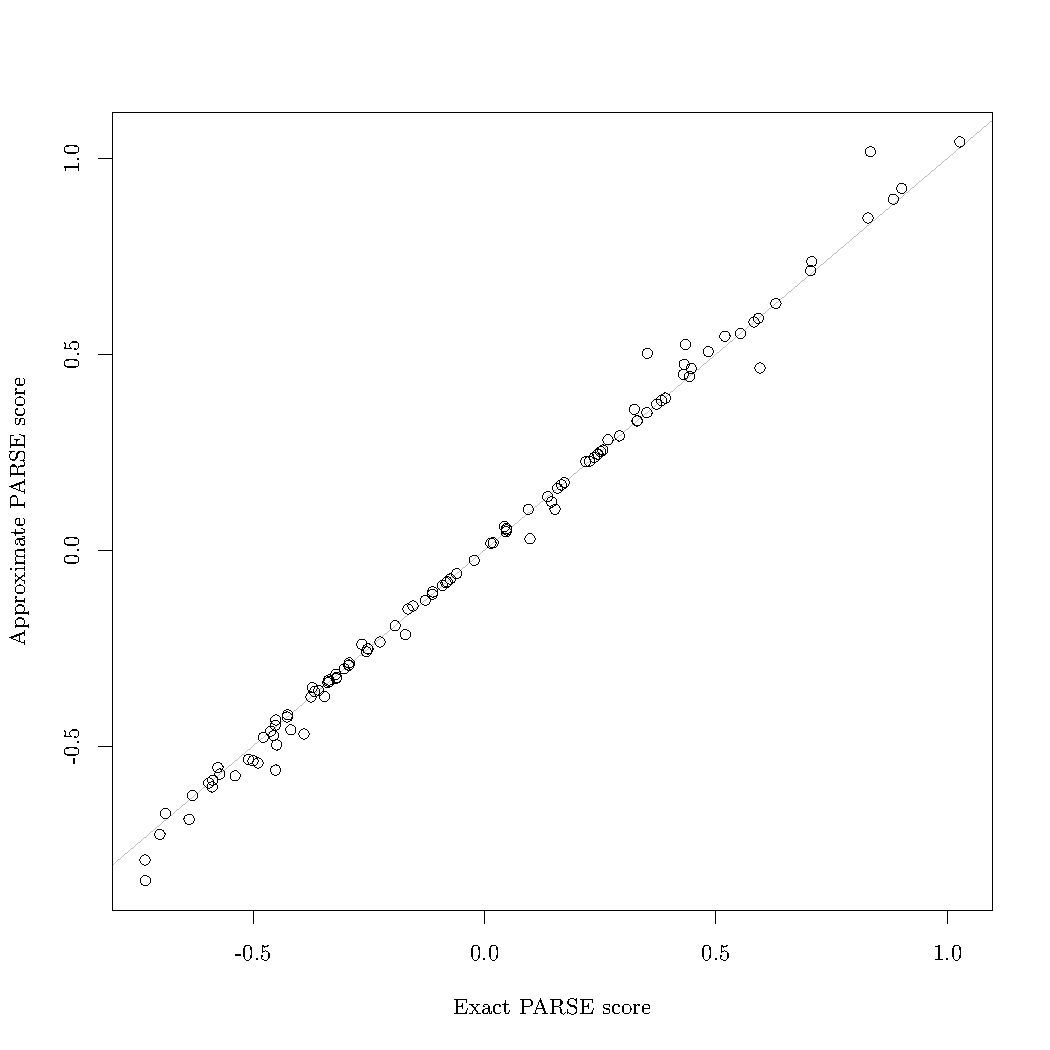
\includegraphics[width=.7\linewidth]{analysis/biosurv/reports/18_SIS_diag_dsd_final/figure/approx-calc-1}
\caption[Performance of the \texorpdfstring{\acrshort{PARSE}}{PARSE} score approximation]{The linear \acrshort{PARSE} score approximation $P \approx k A$ closely matches the exact version calculated using \gls{NNLS}, when evaluated on \gls{APGI} \gls{GEX} data.}\label{fig:app-parse-approx-matching}
\end{figure}

To use the approximation in practice, perform the following steps:
\begin{enumerate}
  \item Prepare a gene $\times$ sample matrix of linear expression estimates $A$, in which values for each row (gene) have been scaled to encompass the range $0$ to $1$.
  \item Subset $A$ to only the genes present in the $k$ vector (\tref{tab:sigs-approx-parse-loadings}), and arrange rows of $A$ so that they exactly match the order of $k$.  If genes present in $k$ are missing from $A$, insert all-zero rows for these genes into $A$.
  \item Calculate approximate \gls{PARSE} scores $P$ as $P = k A$.  This is equivalent to, for each column (sample) of $A$, multiplying each entry of the column of $A$ with the corresponding entry of $k$, and summing the results.
\end{enumerate}

The loading vector for the calculation of approximate \gls{PARSE} score, $k^T$, is given in \tref{tab:sigs-approx-parse-loadings}.

\begin{longtable}[!htbp]{ l r@{.}l @{\hspace{60pt}} l r@{.}l }
\caption[Loading vector for the approximate \texorpdfstring{\acrshort{PARSE}}{PARSE} score]{Loading vector for the approximate \acrshort{PARSE} score.  For brevity and to assist interpretation, this has been split by sign into two columns, but in use both columns should be combined to form a single row vector $k$.}
\label{tab:sigs-approx-parse-loadings}

\hline Gene symbol & \multicolumn{2}{l}{Loading} & Gene symbol & \multicolumn{2}{r}{Loading} \\ \hline
\endfirsthead

\multicolumn{6}{l}{{\bfseries \tablename\ \thetable{} -- continued from previous page}} \\
\hline Gene symbol & \multicolumn{2}{l}{Loading} & Gene symbol & \multicolumn{2}{r}{Loading} \\ \hline
\endhead

\hline \multicolumn{6}{r}{{Continued on next page}} \\
\endfoot

\hline \hline
\endlastfoot

FEM1B & $0$ & $04785$ & GAB2 & $-0$ & $03742$ \\
NCAPG & $0$ & $04487$ & FRZB & $-0$ & $03715$ \\
ANLN & $0$ & $04364$ & MIR99AHG & $-0$ & $03712$ \\
COL12A1 & $0$ & $04098$ & RAP1GAP & $-0$ & $03483$ \\
LDHA & $0$ & $04004$ & NFIA & $-0$ & $03387$ \\
E2F7 & $0$ & $03923$ & TCTA & $-0$ & $03326$ \\
SPHK1 & $0$ & $03861$ & ELMOD3 & $-0$ & $03300$ \\
CEP55 & $0$ & $03755$ & SOBP & $-0$ & $03269$ \\
CHEK1 & $0$ & $03669$ & GIMAP2 & $-0$ & $03176$ \\
TMEM26 & $0$ & $03659$ & STAT5B & $-0$ & $03172$ \\
CKAP2L & $0$ & $03545$ & UFC1 & $-0$ & $03123$ \\
DCBLD2 & $0$ & $03351$ & BOC & $-0$ & $03047$ \\
PHLDA1 & $0$ & $03330$ & P2RY8 & $-0$ & $03043$ \\
KANK4 & $0$ & $03261$ & RNF103 & $-0$ & $03019$ \\
TGFBI & $0$ & $03259$ & KIAA0513 & $-0$ & $02989$ \\
PLAU & $0$ & $03213$ & SGSM1 & $-0$ & $02933$ \\
COL5A3 & $0$ & $03177$ & TOR2A & $-0$ & $02926$ \\
CCNB1 & $0$ & $03071$ & PPY & $-0$ & $02787$ \\
SPOCK1 & $0$ & $03046$ & SH3GL1 & $-0$ & $02784$ \\
ENO2 & $0$ & $02998$ & RPA2 & $-0$ & $02756$ \\
CAV1 & $0$ & $02989$ & SELENBP1 & $-0$ & $02707$ \\
KIF20A & $0$ & $02967$ & TRIM2 & $-0$ & $02689$ \\
RACGAP1 & $0$ & $02957$ & TCEA3 & $-0$ & $02679$ \\
PPAPDC1A & $0$ & $02867$ & HIPK2 & $-0$ & $02620$ \\
RBMS2 & $0$ & $02834$ & CAPN6 & $-0$ & $02615$ \\
RHOF & $0$ & $02828$ & ARHGAP24 & $-0$ & $02524$ \\
CDA & $0$ & $02792$ & TSTD1 & $-0$ & $02503$ \\
NCAPD2 & $0$ & $02756$ & ALDH5A1 & $-0$ & $02452$ \\
MCM4 & $0$ & $02708$ & BCKDK & $-0$ & $02452$ \\
LOX & $0$ & $02695$ & GPC3 & $-0$ & $02419$ \\
PTGES & $0$ & $02681$ & EPHX2 & $-0$ & $02392$ \\
FER & $0$ & $02675$ & DCAF8 & $-0$ & $02374$ \\
EYA3 & $0$ & $02671$ & PPM1H & $-0$ & $02311$ \\
IL20RB & $0$ & $02671$ & PRDM16 & $-0$ & $02289$ \\
GATC & $0$ & $02661$ & MC1R & $-0$ & $02281$ \\
KLHL5 & $0$ & $02641$ & PEX11B & $-0$ & $02280$ \\
ARL4C & $0$ & $02609$ & SMOX & $-0$ & $02258$ \\
ATAD2 & $0$ & $02602$ & LMO3 & $-0$ & $02246$ \\
TPX2 & $0$ & $02590$ & RPIA & $-0$ & $02226$ \\
FGD6 & $0$ & $02545$ & POU2AF1 & $-0$ & $02222$ \\
PRC1 & $0$ & $02492$ & ST3GAL2 & $-0$ & $02187$ \\
MCM10 & $0$ & $02451$ & ZSCAN32 & $-0$ & $02184$ \\
BIRC5 & $0$ & $02419$ & ZFPM1 & $-0$ & $02180$ \\
ZBED2 & $0$ & $02396$ & BCL11B & $-0$ & $02161$ \\
KNTC1 & $0$ & $02375$ & C9orf152 & $-0$ & $02152$ \\
NUP155 & $0$ & $02330$ & SLC40A1 & $-0$ & $02146$ \\
TNFRSF6B & $0$ & $02308$ & CADPS2 & $-0$ & $02136$ \\
HJURP & $0$ & $02296$ & PHOSPHO2 & $-0$ & $02129$ \\
PXDN & $0$ & $02281$ & ST6GAL1 & $-0$ & $02118$ \\
COLGALT1 & $0$ & $02272$ & PLAC9 & $-0$ & $02093$ \\
PLOD2 & $0$ & $02261$ & EIF2AK3 & $-0$ & $02073$ \\
TWIST1 & $0$ & $02246$ & IFT140 & $-0$ & $02068$ \\
RALGAPB & $0$ & $02214$ & CHN2 & $-0$ & $02051$ \\
FSCN1 & $0$ & $02159$ & ZNF658 & $-0$ & $01988$ \\
SPOCD1 & $0$ & $02117$ & MEOX1 & $-0$ & $01961$ \\
SERPINH1 & $0$ & $02086$ & FAM134B & $-0$ & $01945$ \\
GAPDH & $0$ & $02073$ & THSD7B & $-0$ & $01931$ \\
DSG3 & $0$ & $02070$ & TRAPPC2 & $-0$ & $01920$ \\
MELK & $0$ & $02067$ & ADH1A & $-0$ & $01845$ \\
DCUN1D5 & $0$ & $02056$ & LINC01184 & $-0$ & $01837$ \\
TUBA1C & $0$ & $02053$ & SLC12A2 & $-0$ & $01821$ \\
CST6 & $0$ & $02032$ & MRAP2 & $-0$ & $01810$ \\
GABPB1 & $0$ & $01929$ & RASL11B & $-0$ & $01808$ \\
KRT7 & $0$ & $01916$ & RERGL & $-0$ & $01801$ \\
DENND1A & $0$ & $01898$ & PREP & $-0$ & $01799$ \\
AURKB & $0$ & $01869$ & TMTC4 & $-0$ & $01797$ \\
PRR11 & $0$ & $01859$ & TMED1 & $-0$ & $01796$ \\
RFC5 & $0$ & $01848$ & TLE4 & $-0$ & $01794$ \\
SLC16A3 & $0$ & $01842$ & CAMK1G & $-0$ & $01790$ \\
SUGCT & $0$ & $01833$ & GATA6 & $-0$ & $01780$ \\
SCYL2 & $0$ & $01826$ & CCR7 & $-0$ & $01775$ \\
KRT6A & $0$ & $01795$ & SCGB2A1 & $-0$ & $01773$ \\
P4HA2 & $0$ & $01770$ & CCL19 & $-0$ & $01715$ \\
PROSER2 & $0$ & $01761$ & PCF11 & $-0$ & $01710$ \\
PTPN21 & $0$ & $01723$ & FAM189A2 & $-0$ & $01692$ \\
PYGL & $0$ & $01714$ & MCOLN2 & $-0$ & $01684$ \\
GINS2 & $0$ & $01713$ & PLEKHS1 & $-0$ & $01672$ \\
PGBD3 & $0$ & $01700$ & PRMT7 & $-0$ & $01665$ \\
COL7A1 & $0$ & $01688$ & AXIN2 & $-0$ & $01658$ \\
LETM2 & $0$ & $01687$ & TOM1 & $-0$ & $01640$ \\
PDLIM7 & $0$ & $01678$ & RERE & $-0$ & $01635$ \\
KRT17 & $0$ & $01644$ & A4GNT & $-0$ & $01632$ \\
ERRFI1 & $0$ & $01597$ & CDK12 & $-0$ & $01624$ \\
ASPM & $0$ & $01593$ & CNNM1 & $-0$ & $01611$ \\
C1QTNF6 & $0$ & $01572$ & HSPB6 & $-0$ & $01586$ \\
DERA & $0$ & $01568$ & LCNL1 & $-0$ & $01571$ \\
MIF & $0$ & $01560$ & MTRNR2L1 & $-0$ & $01563$ \\
C5orf46 & $0$ & $01559$ & DYNC2H1 & $-0$ & $01537$ \\
EMP3 & $0$ & $01550$ & NPM1 & $-0$ & $01520$ \\
CDK2 & $0$ & $01546$ & CARHSP1 & $-0$ & $01515$ \\
POC1A & $0$ & $01507$ & RGS5 & $-0$ & $01505$ \\
FST & $0$ & $01504$ & CLEC3B & $-0$ & $01500$ \\
KCTD10 & $0$ & $01501$ & NR0B2 & $-0$ & $01468$ \\
SULF2 & $0$ & $01494$ & ARSD & $-0$ & $01466$ \\
CCDC88A & $0$ & $01480$ & GNPAT & $-0$ & $01458$ \\
KIF14 & $0$ & $01477$ & MARS2 & $-0$ & $01442$ \\
DSG2 & $0$ & $01463$ & KCTD5 & $-0$ & $01440$ \\
UHRF2 & $0$ & $01445$ & MRPL24 & $-0$ & $01395$ \\
ZNF185 & $0$ & $01435$ & ABLIM1 & $-0$ & $01392$ \\
SLC2A1 & $0$ & $01424$ & ITPKB & $-0$ & $01390$ \\
KIF2C & $0$ & $01417$ & FHDC1 & $-0$ & $01380$ \\
FLRT3 & $0$ & $01416$ & C2orf70 & $-0$ & $01360$ \\
CNIH3 & $0$ & $01413$ & RAVER2 & $-0$ & $01352$ \\
ITGA5 & $0$ & $01407$ & AKR1A1 & $-0$ & $01321$ \\
DNAJC9 & $0$ & $01385$ & CACHD1 & $-0$ & $01313$ \\
ANGPTL4 & $0$ & $01365$ & ACYP2 & $-0$ & $01298$ \\
KIAA1549L & $0$ & $01354$ & CTSL & $-0$ & $01263$ \\
PPP1R14B & $0$ & $01352$ & TM9SF3 & $-0$ & $01255$ \\
PAX8 & $0$ & $01350$ & PP7080 & $-0$ & $01242$ \\
FAM91A1 & $0$ & $01341$ & IGLL3P & $-0$ & $01241$ \\
EDIL3 & $0$ & $01326$ & ST6GALNAC1 & $-0$ & $01232$ \\
RAB31 & $0$ & $01316$ & VPS35 & $-0$ & $01219$ \\
P2RY2 & $0$ & $01288$ & TAF5L & $-0$ & $01213$ \\
CDC45 & $0$ & $01256$ & STK39 & $-0$ & $01196$ \\
SPIN4 & $0$ & $01254$ & NFIX & $-0$ & $01186$ \\
APCDD1 & $0$ & $01244$ & TNFRSF17 & $-0$ & $01180$ \\
ABHD5 & $0$ & $01227$ & PBXIP1 & $-0$ & $01174$ \\
ANKLE2 & $0$ & $01205$ & PLIN2 & $-0$ & $01174$ \\
FAM83A & $0$ & $01202$ & GOLM1 & $-0$ & $01171$ \\
KYNU & $0$ & $01181$ & SEPW1 & $-0$ & $01161$ \\
ANGPTL2 & $0$ & $01178$ & FYN & $-0$ & $01133$ \\
B3GALTL & $0$ & $01113$ & CA8 & $-0$ & $01129$ \\
MME & $0$ & $01102$ & CSNK1D & $-0$ & $01128$ \\
FAH & $0$ & $01035$ & SLC30A3 & $-0$ & $01126$ \\
NEURL2 & $0$ & $01012$ & SEC23IP & $-0$ & $01125$ \\
CTSV & $0$ & $00987$ & RFK & $-0$ & $01090$ \\
PGAM5 & $0$ & $00973$ & SDIM1 & $-0$ & $01083$ \\
ATL3 & $0$ & $00972$ & ARFGAP3 & $-0$ & $01070$ \\
CD70 & $0$ & $00954$ & CYP2S1 & $-0$ & $01044$ \\
CHAF1B & $0$ & $00920$ & TARBP2 & $-0$ & $01019$ \\
PIGL & $0$ & $00833$ & SERTAD2 & $-0$ & $00995$ \\
PAX8-AS1 & $0$ & $00830$ & IL33 & $-0$ & $00991$ \\
LMTK2 & $0$ & $00804$ & FAM120AOS & $-0$ & $00980$ \\
ACKR3 & $0$ & $00802$ & SYNE2 & $-0$ & $00968$ \\
KRT6C & $0$ & $00798$ & COX4I2 & $-0$ & $00943$ \\
PRKCDBP & $0$ & $00755$ & ANKRD22 & $-0$ & $00941$ \\
DPY19L1 & $0$ & $00749$ & COLGALT2 & $-0$ & $00903$ \\
NACC2 & $0$ & $00733$ & FBXW8 & $-0$ & $00891$ \\
POLA2 & $0$ & $00692$ & MARCKSL1 & $-0$ & $00884$ \\
DKK1 & $0$ & $00649$ & BTN3A1 & $-0$ & $00868$ \\
FBXO22 & $0$ & $00649$ & C1orf56 & $-0$ & $00865$ \\
USP30 & $0$ & $00629$ & PCDH20 & $-0$ & $00861$ \\
APCS & $0$ & $00602$ & EXOSC8 & $-0$ & $00850$ \\
BBS2 & $0$ & $00587$ & AMOT & $-0$ & $00825$ \\
TRERF1 & $0$ & $00581$ & WNT2B & $-0$ & $00812$ \\
GPR176 & $0$ & $00563$ & SLAMF9 & $-0$ & $00761$ \\
FGG & $0$ & $00548$ & PCOLCE2 & $-0$ & $00752$ \\
AKIP1 & $0$ & $00545$ & ZSCAN16 & $-0$ & $00720$ \\
IDH2 & $0$ & $00528$ & CIDECP & $-0$ & $00684$ \\
PFKFB4 & $0$ & $00525$ & BAMBI & $-0$ & $00680$ \\
ANKRD37 & $0$ & $00474$ & IL1R2 & $-0$ & $00660$ \\
SLC2A3 & $0$ & $00438$ & SAMD5 & $-0$ & $00655$ \\
IGFBP1 & $0$ & $00427$ & HSP90B1 & $-0$ & $00641$ \\
A4GALT & $0$ & $00418$ & CFDP1 & $-0$ & $00617$ \\
CEBPB & $0$ & $00404$ & RMND5A & $-0$ & $00614$ \\
PLOD1 & $0$ & $00369$ & CIDEC & $-0$ & $00596$ \\
VSTM2L & $0$ & $00352$ & TPD52L2 & $-0$ & $00579$ \\
XXYLT1 & $0$ & $00341$ & ZNF565 & $-0$ & $00565$ \\
MAP3K8 & $0$ & $00338$ & ACE & $-0$ & $00556$ \\
SNRPB & $0$ & $00276$ & AGRP & $-0$ & $00509$ \\
TOM1L2 & $0$ & $00266$ & PLIN3 & $-0$ & $00506$ \\
NRP2 & $0$ & $00250$ & ARHGEF19 & $-0$ & $00476$ \\
P4HA1 & $0$ & $00225$ & DHRS9 & $-0$ & $00454$ \\
HRASLS2 & $0$ & $00196$ & ATF7IP2 & $-0$ & $00405$ \\
UPP1 & $0$ & $00182$ & NELFE & $-0$ & $00390$ \\
SPP1 & $0$ & $00175$ & RGS3 & $-0$ & $00319$ \\
LAMA5 & $0$ & $00174$ & TNFRSF10D & $-0$ & $00315$ \\
PHACTR3 & $0$ & $00172$ & LOC100506562 & $-0$ & $00290$ \\
ZPLD1 & $0$ & $00165$ & RFX2 & $-0$ & $00264$ \\
CATSPER1 & $0$ & $00163$ & SNORA11D & $-0$ & $00256$ \\
ABHD16A & $0$ & $00143$ & FGB & $-0$ & $00252$ \\
PPP1R3C & $0$ & $00125$ & ICAM2 & $-0$ & $00232$ \\
ADM & $0$ & $00122$ & LGALS9B & $-0$ & $00232$ \\
SOD2 & $0$ & $00120$ & POP5 & $-0$ & $00224$ \\
PPP1R12B & $0$ & $00096$ & NMB & $-0$ & $00205$ \\
NAMPT & $0$ & $00071$ & SERPINB3 & $-0$ & $00201$ \\
KCNQ3 & $0$ & $00040$ & ORC1 & $-0$ & $00199$ \\
MCEMP1 & $0$ & $00025$ & ALOX5AP & $-0$ & $00179$ \\
LYNX1 & $0$ & $00001$ & SLC15A1 & $-0$ & $00139$ \\
\multicolumn{3}{l}{} & OAZ1 & $-0$ & $00134$ \\
\multicolumn{3}{l}{} & TREM1 & $-0$ & $00073$ \\
\multicolumn{3}{l}{} & IKBIP & $-0$ & $00033$ \\
\end{longtable}

\chapter{R code to calculate \texorpdfstring{\acrshort{MSKCC}}{MSKCC} nomogram survival estimates}
\label{app:nomo-mskcc-code}
\begin{lstlisting}[language=R]
fit.mskcc = list(
	inputs = list(
	History.Diagnosis.AgeAt = list(
		margins = data.frame(value = 65, fraction = 1),
		scorefunc = function(x) { x = x; -2/15*pmin(pmax(x, 0), 90) + 12 }),
	Patient.Sex = list(
		margins = data.frame(value = c("M", "F"), fraction = c(0.501, 1-0.501)),
		scorefunc = function(x) { 3*I(x == "M") }),
	Portal.Vein = list(
		margins = data.frame(value = c(TRUE, FALSE), fraction = c(0.144, 1-0.144)),
		scorefunc = function(x) { 10*I(x == TRUE) }),
	Splenectomy = list(
		margins = data.frame(value = c(TRUE, FALSE), fraction = c(0.099, 1-0.099)),
		scorefunc = function(x) { 62*I(x == TRUE) }),
	Treat.MarginPositive = list(
		margins = data.frame(value = c(TRUE, FALSE), fraction = c(0.207, 1-0.207)),
		scorefunc = function(x) { 4*I(x == TRUE) }),
	Path.LocationBody = list(
		margins = data.frame(value = c(FALSE, TRUE), fraction = c(0.894, 1-0.894)),
		scorefunc = function(x) { 51*I(x == TRUE) }),
	Path.Differentiation = list(
		margins = data.frame(value = c("1", "2", "3", "4"), fraction = c(0.142, 0.564, 1-0.142-0.564, 0)),
		scorefunc = function(x) { 14*I(x == "2") + 35*I(x == "3") + 35*I(x == "4") }),		# Undifferentiated (4) not covered by the MSKCC nomogram; here assign the same score as poorly differentiated (3)
	Posterior.Margin = list(
		margins = data.frame(value = c(TRUE, FALSE), fraction = c(0.86, 1-0.86)),
		scorefunc = function(x) { 22*I(x == TRUE) }),
	Path.LN.Involved = list(
		margins = data.frame(value = 2.1, fraction = 1),
		scorefunc = function(x) { 
			x = pmin(40, pmax(x, 0))
			fitfun = splinefun(c(0, 1, 2, 3, 4, 10, 15, 20, 25, 30, 35, 40), c(0, 14.56, 24.64, 30.28, 33.00, 39.05, 43.89, 48.83, 53.77, 58.61, 63.55, 68.49), method = "natural")
			fitfun(x)
		}),
	Path.LN.Negative = list(
		margins = data.frame(value = 16.9, fraction = 1),
		scorefunc = function(x) { (pmin(pmax(x, 0), 90)-90)*-11/90 }),
	Back.pain = list(
		margins = data.frame(value = c(TRUE, FALSE), fraction = c(0.137, 1-0.137)),
		scorefunc = function(x) { 15*I(x == TRUE) }),
	Stage.pT.Simplified = list(
		margins = data.frame(value = c("T1", "T2", "T34"), fraction = c(0.037, 0.119, 1-0.037-0.119)),
		scorefunc = function(x) { 36*I(x == "T1") + 11*I(x == "T34") }),
		# The following matches the original Brennan nomogram, but was not used as there are too few T4
		# tumours in either the NSWPCN *or* the MSKCC cohorts -- how the T4 coefficient was ever estimated,
		# I'll never know.  The T34 coefficient of 11 was arrived at as (0.828*10+(1-0.037-0.119-0.828)*63)/(1-0.037-0.119),
		# being a frequency-weighted average of the T3 and T4 coefficients.
		# margins = data.frame(value = c("T1", "T2", "T3", "T4"), fraction = c(0.037, 0.119, 0.828, 1-0.037-0.119-0.828)),
		# scorefunc = function(x) { 36*I(x == "T1") + 10*I(x == "T3") + 63*I(x == "T4") }),
	Weight.loss = list(
		margins = data.frame(value = c(TRUE, FALSE), fraction = c(0.537, 1-0.537)),
		scorefunc = function(x) { 3*I(x == TRUE) }),
	Path.Size = list(
		margins = data.frame(),
		scorefunc = function(x) {
			x = pmin(16, pmax(x, 0))
			fitfun = splinefun(c(0, 1, 2, 3, 4, 6, 8, 10, 12, 14, 16), c(0, 29.74, 59.48, 86.70, 100, 97.29, 90.03, 82.77, 75.51, 68.25, 61.10), method = "natural")
			fitfun(x)
		}) ),
	outputs = list(
		DSS12mo = function(s) {
			x = pmax(50, pmin(350, s))
			fitfun = splinefun(c(79.0323, 115.02, 165.524, 197.278, 221.774, 242.339, 261.089, 279.839, 299.194, 323.992, 337.298), c(0.94, 0.9, 0.8, 0.7, 0.6, 0.5, 0.4, 0.3, 0.2, 0.1, 0.06))
			y = fitfun(x)
			pmax(0, pmin(1, y))
		},
		DSS24mo = function(s) {
			x = pmax(50, pmin(350, s))
			fitfun = splinefun(c(71.1694, 97.7823, 129.536, 153.73, 174.294, 193.347, 211.794, 231.452, 255.645, 303.125), c(0.86, 0.8, 0.7, 0.6, 0.5, 0.4, 0.3, 0.2, 0.1, 0.01))
			y = fitfun(x)
			pmax(0, pmin(1, y))
		},
		DSS36mo = function(s) {
			x = pmax(50, pmin(350, s))
			fitfun = splinefun(c(69.3548, 101.109, 125.302, 145.867, 164.919, 183.367, 202.722, 226.915, 274.093), c(0.8, 0.7, 0.6, 0.5, 0.4, 0.3, 0.2, 0.1, 0.01))
			y = fitfun(x)
			pmax(0, pmin(1, y))
		}) 
	)

applyNomogram = function(nomogram, data)
{
	scores = rowSums(sapply(names(nomogram$inputs), function(input) {
		if (input %in% colnames(data)) {
			return(nomogram$inputs[[input]]$scorefunc(data[,input]))
		}
		warning(sprintf("Marginalizing missing variable: %s", input))
		margin_score = sum(nomogram$inputs[[input]]$scorefunc(nomogram$inputs[[input]]$margins$value) * nomogram$inputs[[input]]$margins$fraction)
		return(rep(margin_score, nrow(data)))
	}))

	outputs = sapply(nomogram$outputs, function(f) f(scores))
	cbind(Score = scores, outputs)
}
\end{lstlisting}





\chapter{Messina2 Algorithms}
\label{app:mess-algos}

\begin{algorithm}[!htbp]
  \KwData{Covariate measurements $x \in \mathbb{R}^n$, associated dependent values $y \in \mathbb{Y}^n$, objective function $f: (\mathbb{B}^n, \mathbb{Y}^n) \rightarrow \mathbb{B}$, minimum subclass fraction $b \in [0, \frac{1}{2})$, and a number of bootstrap rounds $r$.  $x$ is to be sorted in ascending order.  $\mathbb{Y}$ varies between modes of Messina2.}
  \KwResult{A 3-tuple.  If the fit failed, $(0, 0, 0)$.  Otherwise, optimal classifier parameters $(t^*, d^*, \Delta^*)$, with threshold $t^* \in \mathbb{R}$, direction $d^* \in \{-1, 1\}$, and margin $\Delta^* \in \mathbb{R}^+$.}

  \Begin {
  	$n_{\mathrm{pass}} \longleftarrow 0$\;
  	\For{$i \leftarrow 1$ \KwTo $r$}{
  		\tcp{Generate a bootstrap sample of (x, y)}
  		$(x_{\mathrm{in}}, y_{\mathrm{in}}, x_{\mathrm{out}}, y_{\mathrm{out}}) \longleftarrow \mathrm{BootstrapSample}\left( x, y \right)$\;
  		
  		\tcp{Train Messina2Core on this bootstrap sample}
  		$(t_{\mathrm{in}}, d_{\mathrm{in}}, \Delta_{\mathrm{in}}) \longleftarrow \mathrm{Messina2Core}\left( x_{\mathrm{in}}, y_{\mathrm{in}}, b, f \right)$\;
  		
  		\tcp{Assess performance of the Messina2Core classifier on the out-of-bag samples}
  		\If{$d_{\mathrm{in}} \neq 0$}{
  			$w_\mathrm{out} \longleftarrow \left(~\left[ x_{\mathrm{out}_j} d_{\mathrm{in}} \geq t_{\mathrm{in}} d_{\mathrm{in}}\right]~\right)_{j=1}^{\vert x_\mathrm{out} \vert}$\;
  			\If {$f\left(w_\mathrm{out}, y_{\mathrm{out}}\right) = \mathrm{true}$}{
  				$n_{\mathrm{pass}} \longleftarrow n_{\mathrm{pass}} + 1$\;
  			}
  		}
  	}
  	
  	\tcp{Did the in-bag trained classifiers satisfy out-of-bag performance requirements in at least half of the bootstrap rounds?}
  	\eIf{$r = 0 \vee n_{\mathrm{pass}} \geq \frac{1}{2}r$}{
	  	\tcp{Yes; return the fit on the full data}
  		\KwRet{$\mathrm{Messina2Core}\left( x, y, b, f \right)$}\;
  	}{
  		\tcp{No; this fit failed.}
  		\KwRet{$(0, 0, 0)$}\;
	}
  }
  \caption[Messina2Entry]{Messina2Entry, a bootstrap validation wrapper around Messina2Core.  $\mathrm{BootstrapSample}$ is a function that generates a bootstrap sample of its matched tuple arguments $x$ and $y$, returning both the in-bag and out-of-bag $x$ and $y$ values as tuples.  If the number of bootstrap iterations $r$ is zero, no bootstrap validation is performed and this algorithm falls through to Messina2Core.}
  \label{alg:mess-messina2}
\end{algorithm}

\begin{algorithm}[!htbp]
  \KwData{Covariate measurements $x \in \mathbb{R}^n$, associated dependent values $y \in \mathbb{Y}^n$, minimum subclass fraction $b \in [0, \frac{1}{2})$, and objective function $f: (\mathbb{B}^n, \mathbb{Y}^n) \rightarrow \mathbb{B}$.  $x$ is to be in ascending order.  $\mathbb{Y}$ varies between modes of Messina2.}
  \KwResult{A 3-tuple.  If the fit failed, $(0, 0, 0)$.  If the fit succeeded, optimal classifier values $(t^*, d^*, \Delta^*)$, with threshold $t^* \in \mathbb{R}$, direction $d^* \in \{-1, 1\}$, and margin $\Delta^* \in \mathbb{R}^+$.}

  \Begin {
  	\tcp{Define candidate thresholds $c$ as the midpoints between consecutive unique values of $x$}
  	$c \longleftarrow \mathrm{MakeCutpoints}\left(x, b\right)$\;
  	$m \longleftarrow \vert c \vert$\;
  
	\tcp{Test the objective $f$ on each threshold in $c$}
	\For{$i \leftarrow 1$ \KwTo $m$}{
		$w^+ \longleftarrow \left(~\left[x_j \geq c_i\right]~\right)_{j=1}^n$\;
		$w^- \longleftarrow \left(~\left[x_j < c_i\right]~\right)_{j=1}^n$\;
		$o^+_i \longleftarrow f\left(w^+, y\right)$\;
		$o^-_i \longleftarrow f\left(w^-, y\right)$\;
	}
	
	\tcp{If no threshold passed $f$, return $\varnothing$}
	\If{$o^+ \vee o^-$ is all $\mathrm{false}$}{
      \KwRet $\varnothing$\;
    }
	
	\tcp{Search $o^+$ and $o^-$ for the widest margin contiguous interval that passes $f$}
	$(t^+, \Delta^+) \longleftarrow$ BestInterval$\left(o^+, c\right)$\;
	$(t^-, \Delta^-) \longleftarrow$ BestInterval$\left(o^-, c\right)$\;
	
	\tcp{Return the best of the $o^+$ and $o^-$ results}
	\eIf{$\Delta^+ \geq \Delta^-$}{
	  \KwRet{$(t^+, +1, \Delta^+)$}\;
	}{
	  \KwRet{$(t^-, -1, \Delta^-)$}\;
	}
  }
  \caption[Messina2Core]{Messina2Core.  Searches the real line for the largest interval for which the objective $f(w, y)$ is true, and returns the centre and half-width of that interval.}
  \label{alg:mess-core}
\end{algorithm}

\begin{algorithm}[!htbp]
  \KwData{Covariate measurements $x \in \mathbb{R}^n$, and a minimum subclass fraction $b \in [0, \frac{1}{2})$.  $x$ is to be sorted in ascending order.}
  \KwResult{A tuple of candidate cutpoints $c$, with values sorted in ascending order.}

  \Begin {
  	$x' \longleftarrow \mathrm{unique}(x)$\;
  	$c \longleftarrow ()$\;
  	\For{$i \leftarrow 1$ \KwTo $\vert x' \vert - 1$}{
  		$p \longleftarrow \frac{1}{2} \left({x'}_i + {x'}_{i+1}\right)$\;
  		$s \longleftarrow \frac{1}{n} \sum_{i=1}^n \left[ x_i < p \right] $\;
  		\If{$s \geq b \wedge s \leq 1-b$}{
	  		$c \longleftarrow c \oplus p$\;
	  	}
  	}
  	\If{$b = 0$}{
	  	$c \longleftarrow -\infty \oplus c \oplus \infty$\;
	}
  	
	\KwRet{$c$}\;
  }
  \caption[MakeCutpoints]{MakeCutpoints.  Returns a sorted list of candidate cutpoints, each dividing the values in $x$ into two groups, with the restriction that all groups must contain at least fraction $b$ of the original values of $x$.  The function $\mathrm{unique}$ accepts a tuple argument, and returns a tuple containing the unique values of its argument, in ascending order.  The symbol $\oplus$ is used to represent tuple concatenation, and $()$ is the empty tuple.}
  \label{alg:mess-cutpoints}
\end{algorithm}

\begin{algorithm}[!htbp]
  \KwData{$o \in \mathbb{B}^m$, $c \in \mathbb{R}^m$, $x \in \mathbb{R}^n$}
  \KwResult{$(t^* \in \mathbb{R}, \Delta^* \in \mathbb{R}^+)$}

  \Begin {
    $\Delta^* \longleftarrow 0$\;
    $t^* \longleftarrow 0$\;
    
    $i \longleftarrow 1$\;
    \While{$i \leq m$}{
      \If{$o_i$ is $\mathrm{true}$}{
        $r_L \longleftarrow \sup \{x_k~|~x_k \leq c_i \wedge k \in \mathbb{N}^+ \wedge k \leq n \}$\;
        \For{$j \leftarrow i$ \KwTo $m$}{
          \eIf{$o_j$ is $\mathrm{true}$}{
            $r_R \longleftarrow \sup \{x_k~|~x_k \leq c_j \wedge k \in \mathbb{N}^+ \wedge k \leq n \}$\;
          }{
            break\;
          }
        }

		$\Delta \longleftarrow \frac{1}{2}\left(r_R - r_L\right)$\;
        \If{$\Delta > \Delta^*$}{
          $\Delta^* \longleftarrow \Delta$\;
          $t^* \longleftarrow r_L + \frac{1}{2}\Delta$\;
        }
        
        $i \longleftarrow j$\;
      }
      $i \longleftarrow i + 1$\;
    }
    \KwRet{$(t^*, \Delta^*)$}\;
  }
  
  \caption[BestInterval]{BestInterval.  Identifies the centre ($t^*$) and half-width ($\Delta^*$) of the largest interval on $t$ for which $o(t) = true$.  $o$ is only sampled at values in $c$, but changes value only at values in $x$; the process by which this algorithm translates between these representations is illustrated in \fref{fig:mess-bestinterval}.}
  \label{alg:mess-bestinterval}
\end{algorithm}

\begin{figure}[!hp]
\centering
\begin{tikzpicture}[
    axis/.style={thick,<->,>=stealth},
    guide/.style={thick,dotted,gray},
    graphline/.style={thick,black},
    threshmark/.style={thin,->,>=stealth}]

  \def\f{*0.6}

  \draw[axis]
    (1\f,2\f) -- (16\f,2\f);

  \draw[guide]
    (1\f,3\f) -- (16\f,3\f)
    (1\f,6\f) -- (16\f,6\f);

  \draw[graphline,<-,>=stealth]
    (1\f,3\f) -- (4.5\f,3\f);
  \draw[graphline,->,>=stealth]
    (13\f,3\f) -- (16\f,3\f);
  \draw[graphline]
    (4.5\f,6\f) -- (7\f,6\f)
    (7\f,3\f) -- (9\f,3\f)
    (9\f,6\f) -- (13\f,6\f);

  \filldraw[black,draw=black] (2\f,3\f) circle [radius=0.1\f];
  \filldraw[black,draw=black] (3\f,3\f) circle [radius=0.1\f];
  \filldraw[black,draw=black] (4.5\f,6\f) circle [radius=0.1\f];
  \filldraw[black,draw=black] (6\f,6\f) circle [radius=0.1\f];
  \filldraw[black,draw=black] (7\f,3\f) circle [radius=0.1\f];
  \filldraw[black,draw=black] (9\f,6\f) circle [radius=0.1\f];
  \filldraw[black,draw=black] (13\f,3\f) circle [radius=0.1\f];
  \filldraw[black,draw=black] (14.5\f,3\f) circle [radius=0.1\f];
  \filldraw[black,draw=black] (15\f,3\f) circle [radius=0.1\f];
  \filldraw[white,draw=black] (4.5\f,3\f) circle [radius=0.1\f];
  \filldraw[white,draw=black] (7\f,6\f) circle [radius=0.1\f];
  \filldraw[white,draw=black] (9\f,3\f) circle [radius=0.1\f];
  \filldraw[white,draw=black] (13\f,6\f) circle [radius=0.1\f];

  \draw[threshmark] (1.5\f,1.5\f) -- (1.5\f,1.95\f);
  \draw[threshmark] (2.5\f,1.5\f) -- (2.5\f,1.95\f);
  \draw[threshmark] (3.75\f,1.5\f) -- (3.75\f,1.95\f);
  \draw[threshmark] (5.25\f,1.5\f) -- (5.25\f,1.95\f);
  \draw[threshmark] (6.5\f,1.5\f) -- (6.5\f,1.95\f);
  \draw[threshmark] (8\f,1.5\f) -- (8\f,1.95\f);
  \draw[threshmark] (11\f,1.5\f) -- (11\f,1.95\f);
  \draw[threshmark] (13.75\f,1.5\f) -- (13.75\f,1.95\f);
  \draw[threshmark] (14.75\f,1.5\f) -- (14.75\f,1.95\f);
  \draw[threshmark] (15.5\f,1.5\f) -- (15.5\f,1.95\f);

  \node[align=left] at (1.5\f,1.2\f) {\tiny $c_1$};
  \node[align=left] at (2.5\f,1.2\f) {\tiny $c_2$};
  \node[align=left,text width=10\f] at (3.75\f,1.2\f) {\tiny $c_3...$};
  \node[align=left,text width=10\f] at (11\f,1.2\f) {\tiny $t^*$};

  \node[align=right,text width=30\f] at (-0.5\f,2\f) {\footnotesize $t$};
  \node[align=left,text width=30\f] at (-0.5\f,3\f) {\scriptsize 0};
  \node[align=left,text width=30\f] at (-0.5\f,6\f) {\scriptsize 1};

  \draw 
    (-1.5\f,2.5\f) -- (-1.75\f,2.5\f)
    (-1.75\f,2.5\f) -- (-1.75\f,6.5\f)
    (-1.5\f,6.5\f) -- (-1.75\f,6.5\f);

  \node at (-3\f,4.5\f) {\footnotesize $o$};

  \draw[decorate,decoration={brace,amplitude=10\f},rotate=0] (9\f,7\f) -- (13\f,7\f);

  \node[align=center] at (5.75\f,6.5\f) {\scriptsize Region 1};
  \node[align=center] at (11\f,6.5\f) {\scriptsize Region 2};
  \node[align=center] at (11\f,7.75\f) {\scriptsize $2\Delta^*$};
\end{tikzpicture}
\caption[Operation of the BestInterval algorithm]{Operation of the BestInterval algorithm.  Example values of a binary objective $o$ are shown for a range of input thresholds $t$.  $o$ is a sparse sample of the objective function $f$, evaluated at candidate cutpoints $c$, $o_i = f(w(c_i,d),y)$.  At discrete points defined by observed data values (shown as dots), the objective function $f$ can transition, as an observed data point changes its value relative to $t$, and therefore its assigned class.  Two regions in which $o = 1$ are shown.  BestInterval locates all such regions, selects the one with largest measure on $t$ (margin), and returns its centre and margin as $(t^*, \Delta^*)$.  In this example, the centre and margin of region 2 would be returned.  To ensure that $o$ is sampled at sufficient density, candidate thresholds $c_1, c_2, \dots$ are defined between all consecutive values, and beyond the extrema, of $x$; these are indicated by small arrows.}
\label{fig:mess-bestinterval}
\end{figure}


\backmatter

\printglossary

\renewcommand{\bibname}{References}
\bibliographystyle{abbrv}
\bibliography{dissertation}

\end{document}
